\documentclass[../Head/Main.tex]{subfiles}
\begin{document}
\section{Robotics}
\label{sub:Robotics}
This section will explain in detail the robotics part of this project. Moreover, which hardware are used on the drone, how the offboard controller node is working, to automatically move the drone between waypoints. This was developed and tested in a simulated environment using Gazebo.

\subsection{Hardware}
\label{subsec:hardware}
A small overview of the drone and hardware components needed on a very high level can be seen in \autoref{fig:drone_img} and \autoref{fig:hardware_overview}.

\begin{figure}[H]
    \centering
    \begin{subfigure}[t]{.43\textwidth}
        \centering
        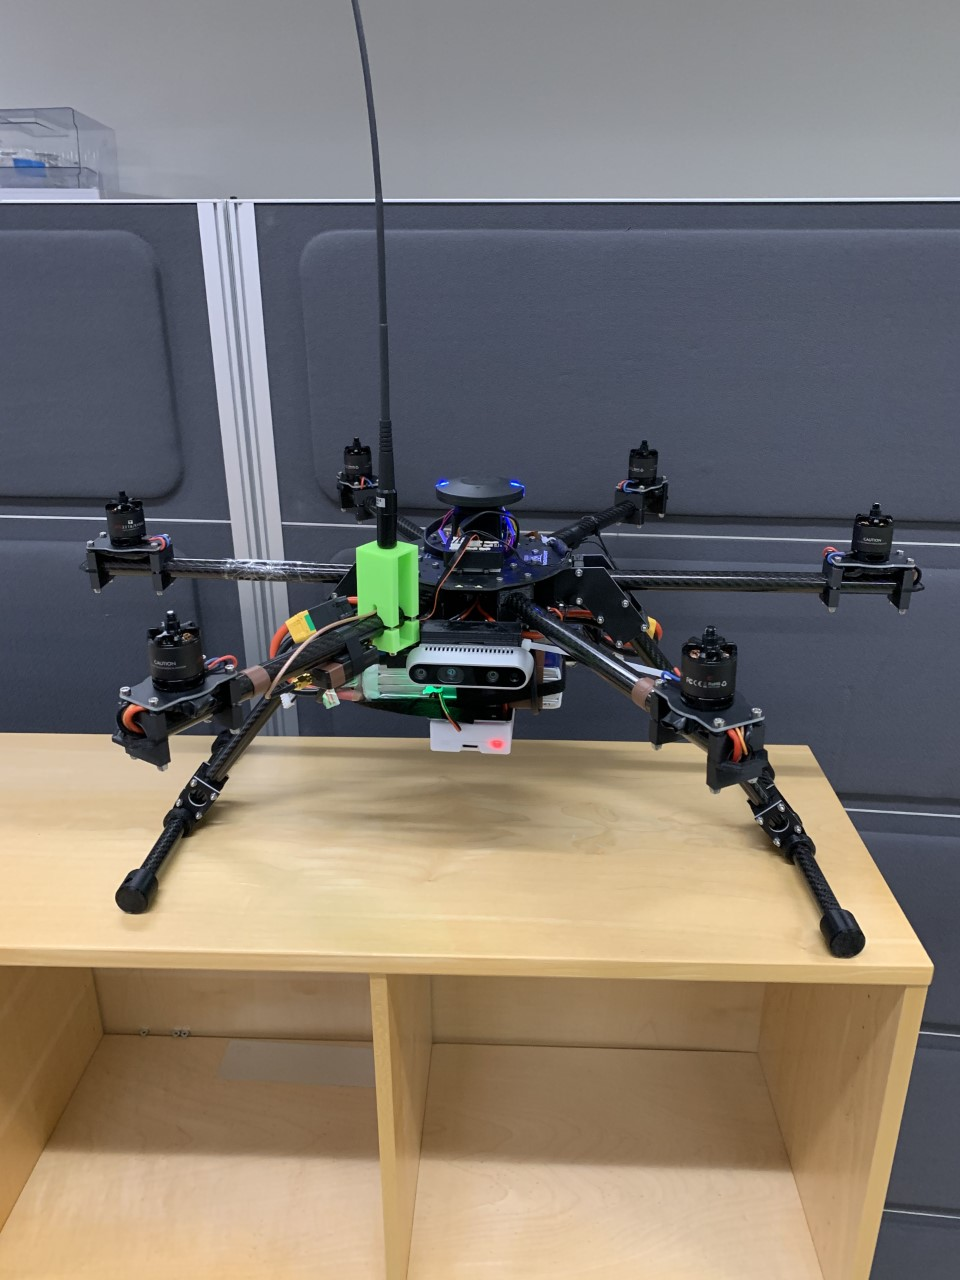
\includegraphics[width=\textwidth]{../Figures/drone.jpeg}
        \caption{Image of the drone with mounted camera}
        \label{fig:drone_img}
    \end{subfigure}
    \hfill
    \begin{subfigure}[t]{.45\textwidth}
        \centering
        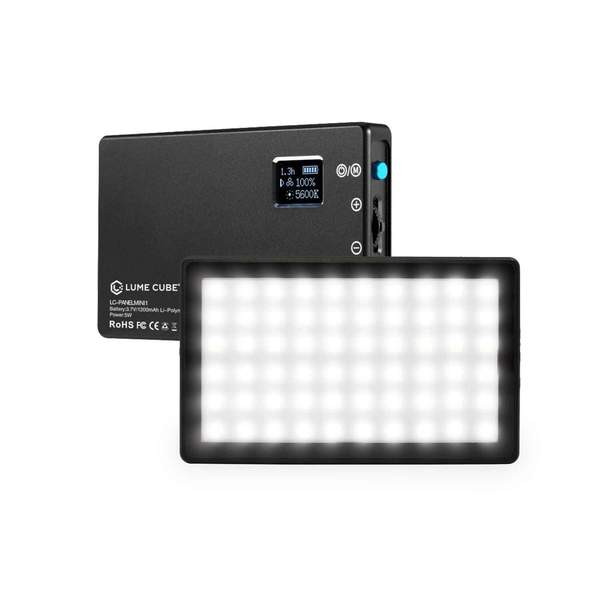
\includegraphics[width=\textwidth]{../Figures/panel-mini-back-front_600x.jpg}
        \caption{Lume Cube Panel Mini \cite{Lume_cube_mini}}
        \label{fig:fig:lume_cube_panel_mini}
    \end{subfigure}
    \caption{Illustrations of the drone and Lume cube}
\end{figure}

Furthermore a Lume cube panel mini had been placed underneath the drone to make it able to illuminate the fence when it gets dark, this will ensure that the vision algorithm is still able to get some nice data during darkness \cite{Lume_cube_mini}.\\
This small piece of hardware, has a very nice illumination range and is very bright, meanwhile it is very lightweight. An illuminated image can be seen in \autoref{fig:image_light_projected}.

\begin{figure}[H]
    \centering
    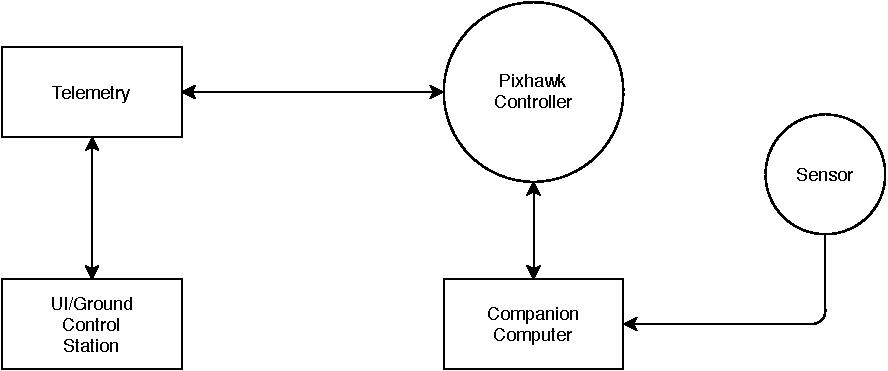
\includegraphics[width=0.8\textwidth]{../Figures/hardware_overview.pdf}
    \caption{Overview of the different hardware components.}
    \label{fig:hardware_overview}
\end{figure}

In \autoref{fig:hardware_overview} an overview of the connected hardware are visualised. The sensor is directly fed through an USB to the raspberry PI model 3 B+ which then talks to the Pixhawk with the use of MavRos. A pair of telemetry antennas are used, with TX on the drone and the receiving unit e.g. on a laptop which enables communication and status updates on the drone while it is flying through e.g. QGroundControl.  

\clearpage
\subsection{Simulation and Software}
\label{subsec:simulation}
Initially, a Gazebo server and client was set up to emulate the drone, fence and the different sensors. To ensure that the drone would be able to do autonomous flight and inspection, a ROS framework to control the drone was designed that could also handle the sensors put on the drone.\par 
The ROS framework was based upon a modular structure, drawing inspiration from behaviour based robotics and the fundamental structure of ROS. The structure was based on a core, a message handler and distributed nodes with specialised functionality. 
A graphical representation of the framework can be seen in \autoref{fig:ros_framework}.

\begin{figure}[H]
    \centering
    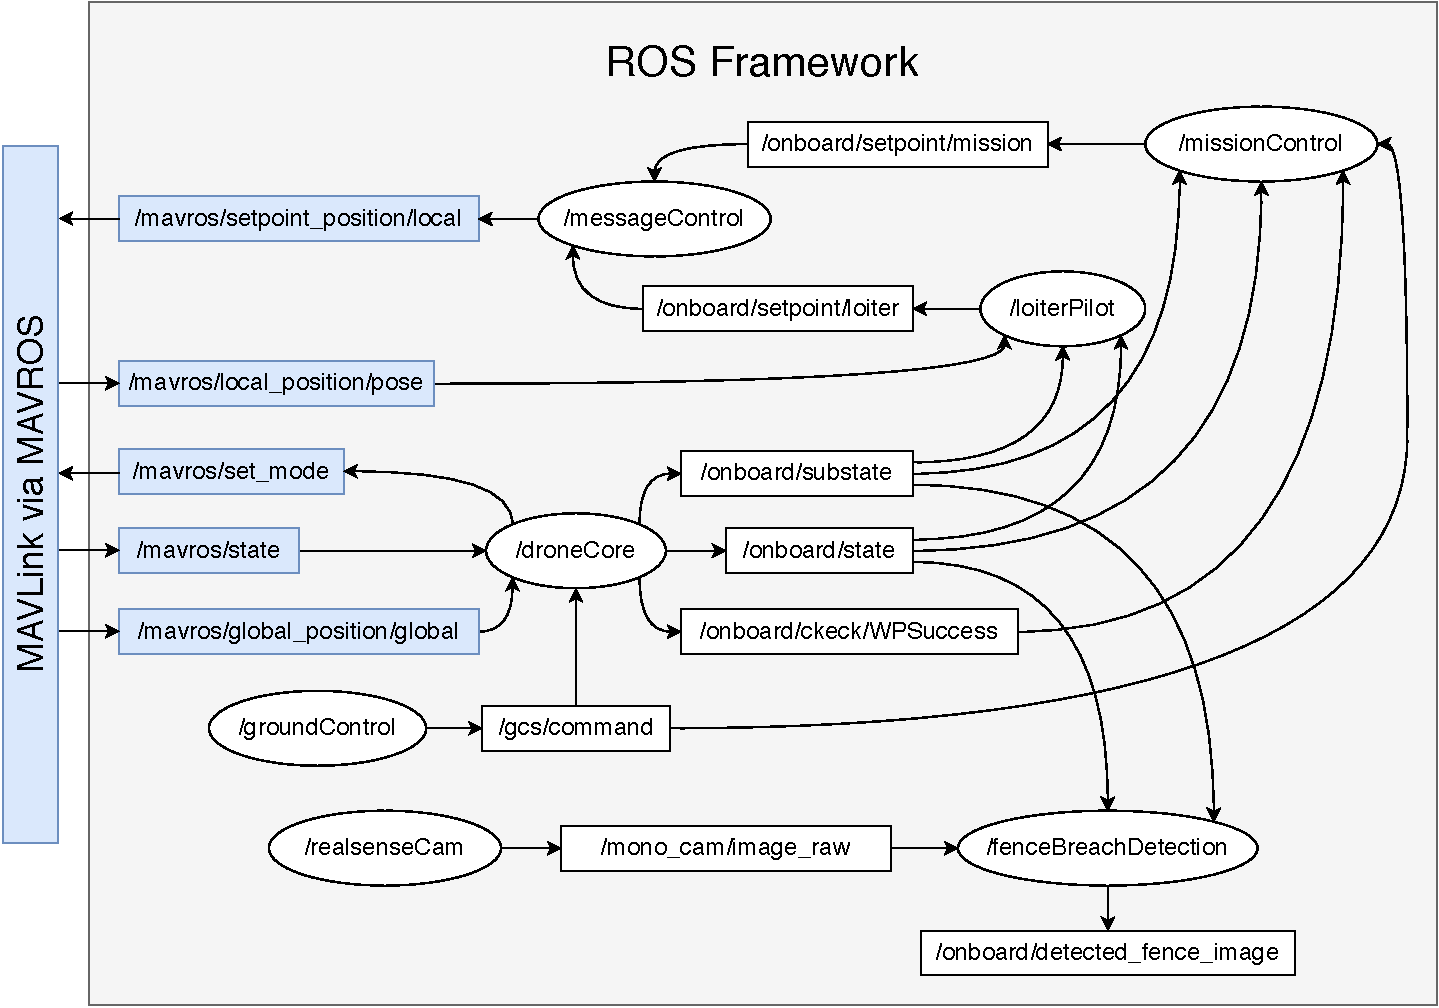
\includegraphics[width=\textwidth]{../Figures/simulation/ROS_framework.pdf}
    \caption{ROS framework for the Gazebo simulation}
    \label{fig:ros_framework}
\end{figure}

The oval and rectangular elements of \autoref{fig:ros_framework} represent ROS nodes and ROS topics respectively. The design consists of two main nodes that handles the core functionality of the framework. The dronecore and messageControl node, these nodes were designed to be the only nodes that could write to the PX4 related topics, where all nodes could read from those topics. This idea was considered to reduce the number of nodes that talks to the PX4 and give a clear separation between the PX4 and companion computer. This means that all nodes that would like to give positional information to the PX4 would have to be forwarded though the messageControl node. This will add a little more computational complexity to the system, but will enable the system to fully control what nodes are able to talk to the PX4 while also having access to different kinds of positional information. This could be beneficial if a waypoint needs to be corrected based on the distance to the fence. Meaning that it would be easy to add deviations to the flight paths. \par

\clearpage
\textbf{droneCore:} This node was designed to be the only node that could change settings on the PX4 flight controller and handles all state changes for both the PX4 and companion computer. It also takes commands from the ground control station, and contains core functionalities like takeoff, PX4 based landings and writes to the topic \textit{/onboard/WPComplete} if a waypoint have been reached. \par
A basic state machine was designed to handle different scenarios of drone flight seen in \autoref{fig:ROS_FSM}. 
\begin{figure}[H]
    \centering
    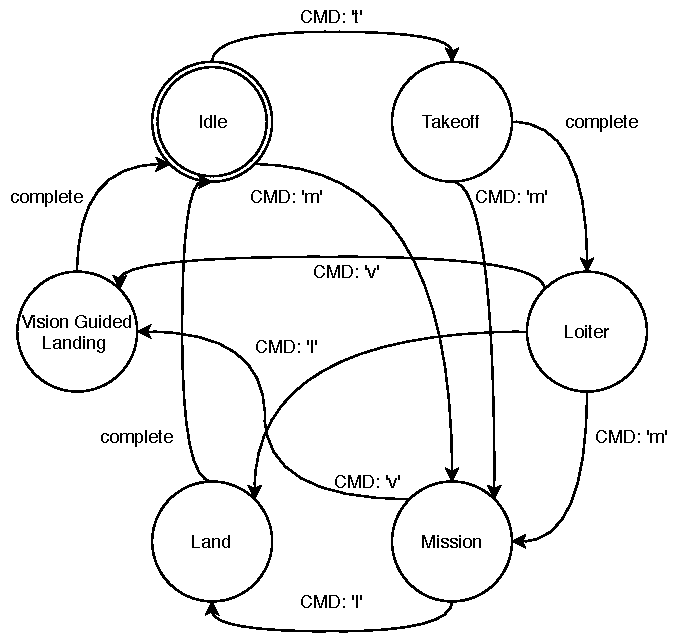
\includegraphics[width=0.75\textwidth]{../Figures/simulation/ROS_framwork_FSM.pdf}
    \caption{Illustration of the finite state machine for the drone companion computer}
    \label{fig:ROS_FSM}
\end{figure}
The state machine for the droneCore node can be seen on \autoref{fig:ROS_FSM}. The state machine has six states; when the PX4 flight controller has the control of the drone (idle mode), a takeoff state to perform an automated takeoff, automated landing state, a loiter state where the loiter pilot will be enabled, a mission state where a mission will be executed and vision guided landing state where an autonomous vision based precision landing will be performed.\\
The vision guided landing feature was not intended to be something that would be implemented but preparing the system for the feature would make implementation easier.\\
The commands that initiate state transitions are commands from the ground control station. The commands will be discussed in combination with the ground control node below.

\textbf{LoiterPilot:}
This node was designed to enable to drone to loiter while in offboard mode. The node takes advantage of the PX4 position hold functionality, and only resends the local position setpoint as the PX4 would otherwise think that companion computer have died. If it dies it will deploy a fail-safe routine. It was implemented with additional functions to alter the position of the drone for easy debugging in simulation. The following functions were implemented; moving along the x, y and z axis in increments of 0.5 m, and yaw rotation of the drone. The axis movement does not take the drones orientation into account. 
\par 

\clearpage
\textbf{MissionControl:}
This node was designed to execute a mission. Although the PX4 is capable of executing a mission it only specifies a flight path and some additional features was needed to perform an inspection. The idea was that a mission would be written as a file of commands, that would be executed. The following commands where added to the mission control node. \textit{COMMAND} for performing a command. Could either be a ground control based command like takeoff/land or an internal command like start recording. \textit{STATE} for changing the onboard state. \textit{SUBSTATE} for changing the onboard substate like enabling a vision algorithm. \textit{PARAM} for updating a PX4 parameter, e.g. max velocity. \textit{WAYPOINT} for giving a waypoint to navigate to. Confirmation that the drone have moved in position will come from the droneCore. This was implemented using local coordinates and quaternions, but it was intended to be based on global GPS coordinates in a final version.\\
This node implements the same basic functionality of loiter pilot. One of the reasons for duplicating some of the functionality of the nodes, was to ensure that the droneCore could enable a different node and continue to have control over the drone if the current node crashes. If parts of the mission control crashes the loiter pilot would take over and keep the drone in the air at the current location. If everything fails then the PX4 will enable a fail-safe routine, e.g. land.
In \autoref{fig:FSM_MSSN}, the state machine for the mission control node can be seen. It contains a state for each command, an idle state, a state that waits for a given state change, a state that waits for being in position and a state for fetching the next command. The only two states that does not lead directly back to fetching the next commands are send command and set waypoint, as these commands require a wait state. If a takeoff is being performed with a send command, then the mission control will wait for the system to change into loiter mode.
\begin{figure}[H]
    \centering
    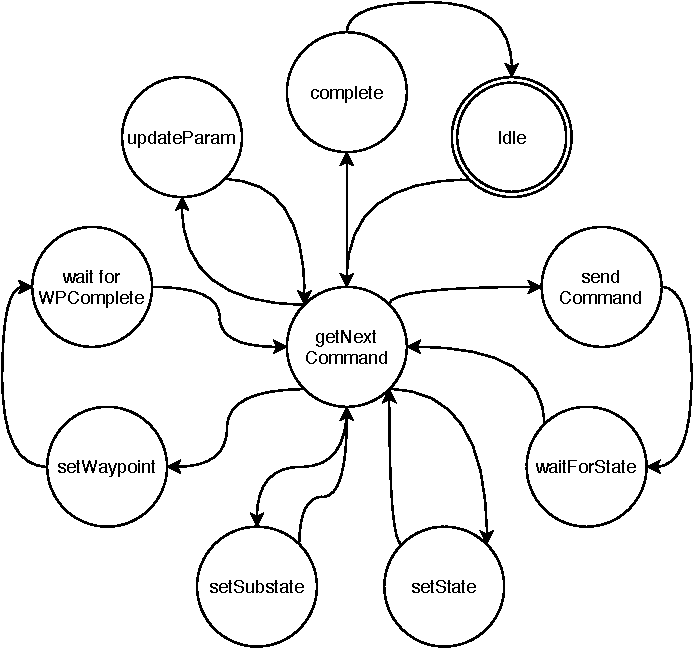
\includegraphics[width=0.7\textwidth]{../Figures/simulation/missionControlFSM.pdf}
    \caption{Finite state machine for mission control via the companion computer}
    \label{fig:FSM_MSSN}
\end{figure}
\par 

\clearpage 
\textbf{MessageControl:}
This node was designed to relay all positional inputs from the different control nodes to the PX4, based on the overall state off the system. This architecture was chosen to ensure that as few node as possible have write access to the drones flight controller. This setup also enables the node to see if the current controller node is outputting positional information, and uses those topics as heartbeat signals for the controller nodes. If the current controller stops responding, the control will be given to the loiter pilot. This feature was added to give the companion computer time to resolve itself while being in control of the drone and only handing over the control of the drone to a PX4 fail-safe if necessary. Any functionality to restart a node was not implemented but intended to be a part of the droneCore node.   
\par 

\textbf{GroundControl:}
This node was designed to emulate a ground control station in the simulation. The node would take inputs from the keyboard and send them to the companion computer. This could be implemented on a drone with a telemetry link and some additional security to minimise the risk of hijacking. The commands that the drone can receive from the ground control node can be seen in \autoref{tab:ROS_commands}.
\begin{table}[H]
\centering
\begin{tabular}{ll}
\hline
\textbf{Keypress} & \textbf{Action}                                    \\ \hline
t                 & droneCore: takeoff + offboard + loiter mode        \\
o                 & droneCore: offboard + loiter mode                  \\
v                 & droneCore: vision guided landing (not implemented) \\
m                 & droneCore: mission                                 \\
h                 & droneCore: move the drone to home and land         \\
k                 & droneCore: kill switch (not implemented)           \\
r                 & droneCore: reset ROS framework (not implemented)   \\
l                 & droneCore: land at current location                \\
                  &                                                    \\
wasd              & loiterpilot: forwards, left, back, right           \\
qe                & loiterpilot: yaw ccw/cw (respectively)             \\
zx                & loiterpilot: decrease/increase altitude           
\end{tabular}
\caption{Table of all possible commands from ground control station}
\label{tab:ROS_commands}
\end{table}
The commands given to the companion computer was implemented with characters to make easy use of the keyboard.
\par 

\textbf{RealsenseCam:}
This node was designed to function as a driver for the Intel Realsense camera and publishes the image data to a ROS topic. It also does a little pre-processing to get a depth image from the depth information that the camera gives. If software for adaptable camera settings will be needed it would be implemented in this node. 
\par 

\textbf{FenceBreachDetection:}
This node was designed to be the node for detecting fence breaches. An Fast Fourier Transformation (FFT) based detection approach was implemented in this node originally, that was able to run real-time on the Raspberry Pi. See \autoref{seg:fouier_transformation}.\\ 
A more advanced deep-learning based approach have also been looked at, which would probably be too heavy computationally for the Raspberry Pi if run real-time. Therefore the approach for that solution would be to save the data and post-process it after landing.\\
An additional solution to this have been considered to enable real-time performance with an AI based approach. This solution requires some additional computational power for the AI inference model based on an Intel Neural Compute Stick 2.
\clearpage
In \autoref{fig:NCS2} an illustration of the Intel Neural Compute Stick 2 can be seen. It is a small portable computational stick that are specially developed for deep-learning inference. It features a Movidius Myriad X Vision Processing Unit (VPU) with 16, 700 MHz SHAVE cores, that according to Intel are special CPUs with an instruction set tailored for deep neural nets and with a price of 595 DKK it was found to be a very capable device  \cite{Intel_NCS2_spec,Intel_NCS2_VPU_spec,Intel_NCS2_price}.\\
It can be used with an Raspberry by running Ubuntu and a Tensorflow based inference model. An illustration of this can be seen in \autoref{fig:NCS2_RPi}. Additional sticks can be added to the system for additional computational power.

\begin{figure}[H]
    \centering
    \begin{subfigure}{0.49\textwidth}
        \vspace{25pt}
        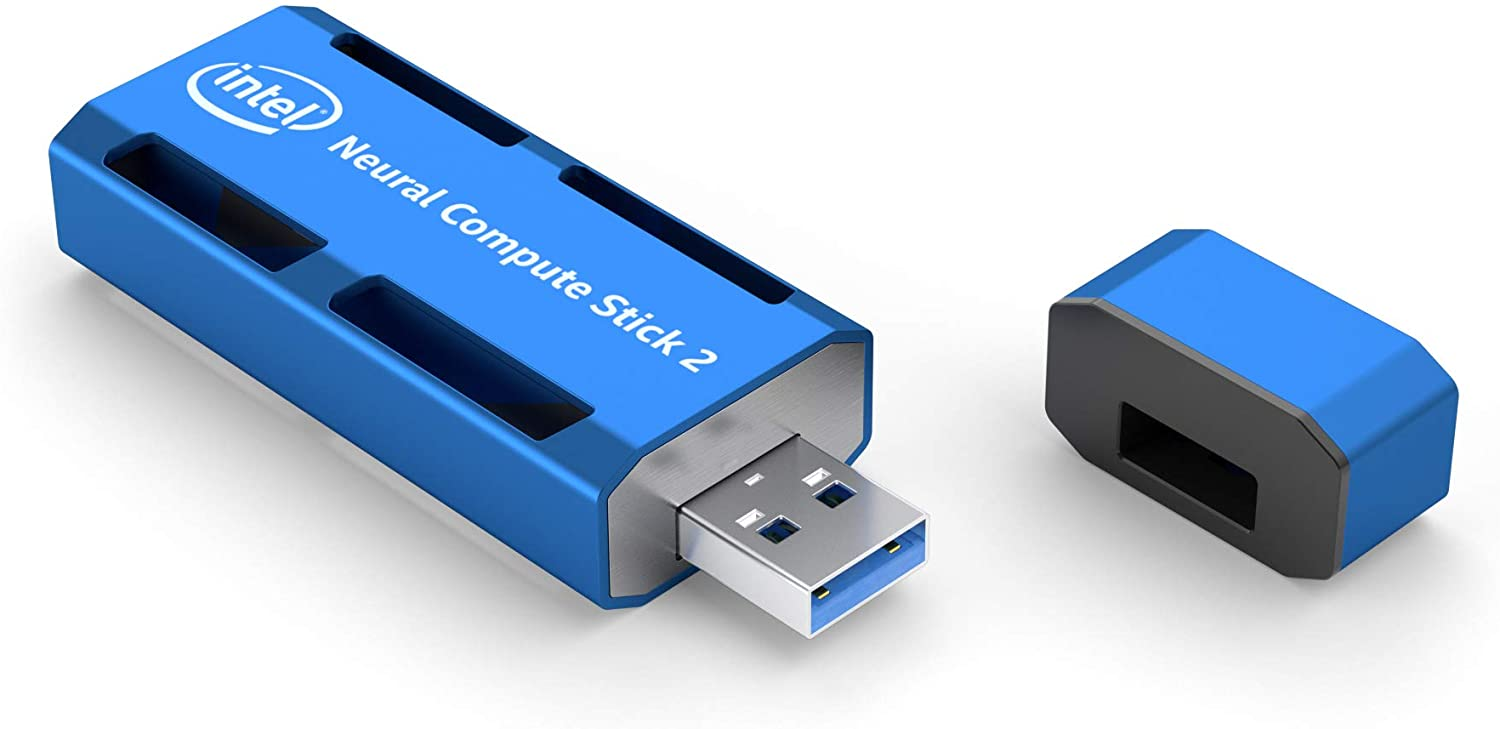
\includegraphics[width=\textwidth]{../Figures/Intel_NCS2.jpg}
        \vspace{25pt}
        \caption{Illustration of the Intel Neural Compute Stick 2. It is the size of a large USB thumb drive \cite{Intel_NCS2_IMG}}
        \label{fig:NCS2}        
    \end{subfigure}
    \hfill
    \begin{subfigure}{0.49\textwidth}
        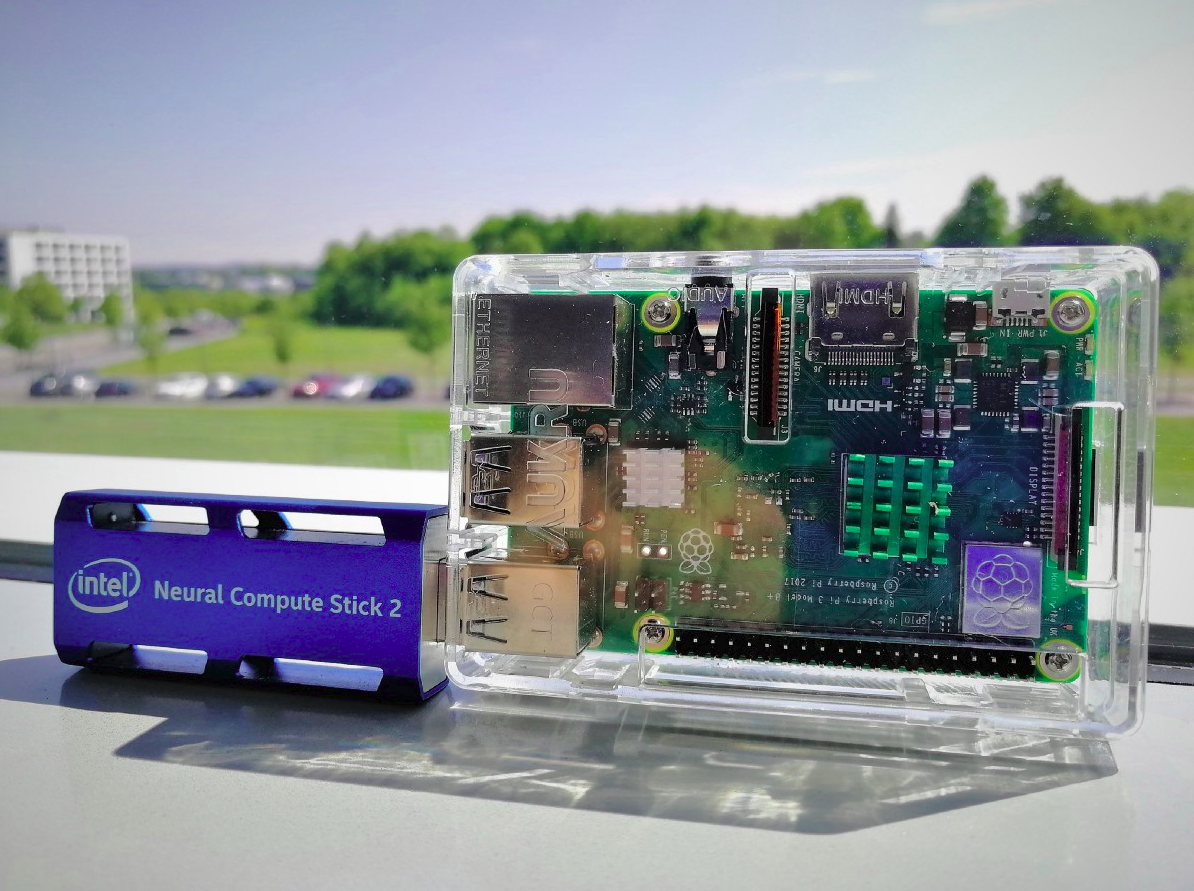
\includegraphics[width=\textwidth]{../Figures/Intel_NCS2_RPi.png}
        \caption{Illustration of the Intel Neural Compute Stick 2 with a Raspberry Pi 3B+ \cite{Intel_NCS2_IMG_RPi}}
        \label{fig:NCS2_RPi}        
    \end{subfigure}
    \caption{Intel Neural Compute Stick 2}
    \label{fig:Intel_NCS2}
\end{figure}

\subsection{Final simulation test}
Here a final simulation test will be documented. A simple fence was added to the optitrack Gazebo world, and a simple mission was written to arm and takeoff the drone. Then fly to the left of the fence, start the fence inspection, and setting the maximum xy velocity to 1 m/s to ensure smooth fly by. Thereafter flying the drone to the right of the fence, resetting velocity settings and returning home to land. The mission file used can be seen below.

\begin{lstlisting}
COMMAND;t;loiter
STATE;mission
WAYPOINT;-5.0;-1.0;1.0;0.0;0.0;90.0
SUBSTATE;fence_breach_detection
PARAM;MPC_XY_VEL_MAX;1.0
WAYPOINT;5.0;-1.0;1.0;0.0;0.0;90.0
SUBSTATE;idle
PARAM;MPC_XY_VEL_MAX;12.0
PARAM;MPC_VEL_MANUAL;10.0
WAYPOINT;0.0;0.0;1.0;0.0;0.0;0.0
COMMAND;l;land
COMPLETE
\end{lstlisting}

In \autoref{fig:SIM_flight} illustrations of the simulated flight can be seen with the drone taking off, moving left, slowly moving right and then returning to land.

\newcommand{\figSize}{0.33\textwidth}

\begin{figure}[h]
    \centering
        \begin{subfigure}{\figSize}
            \centering
            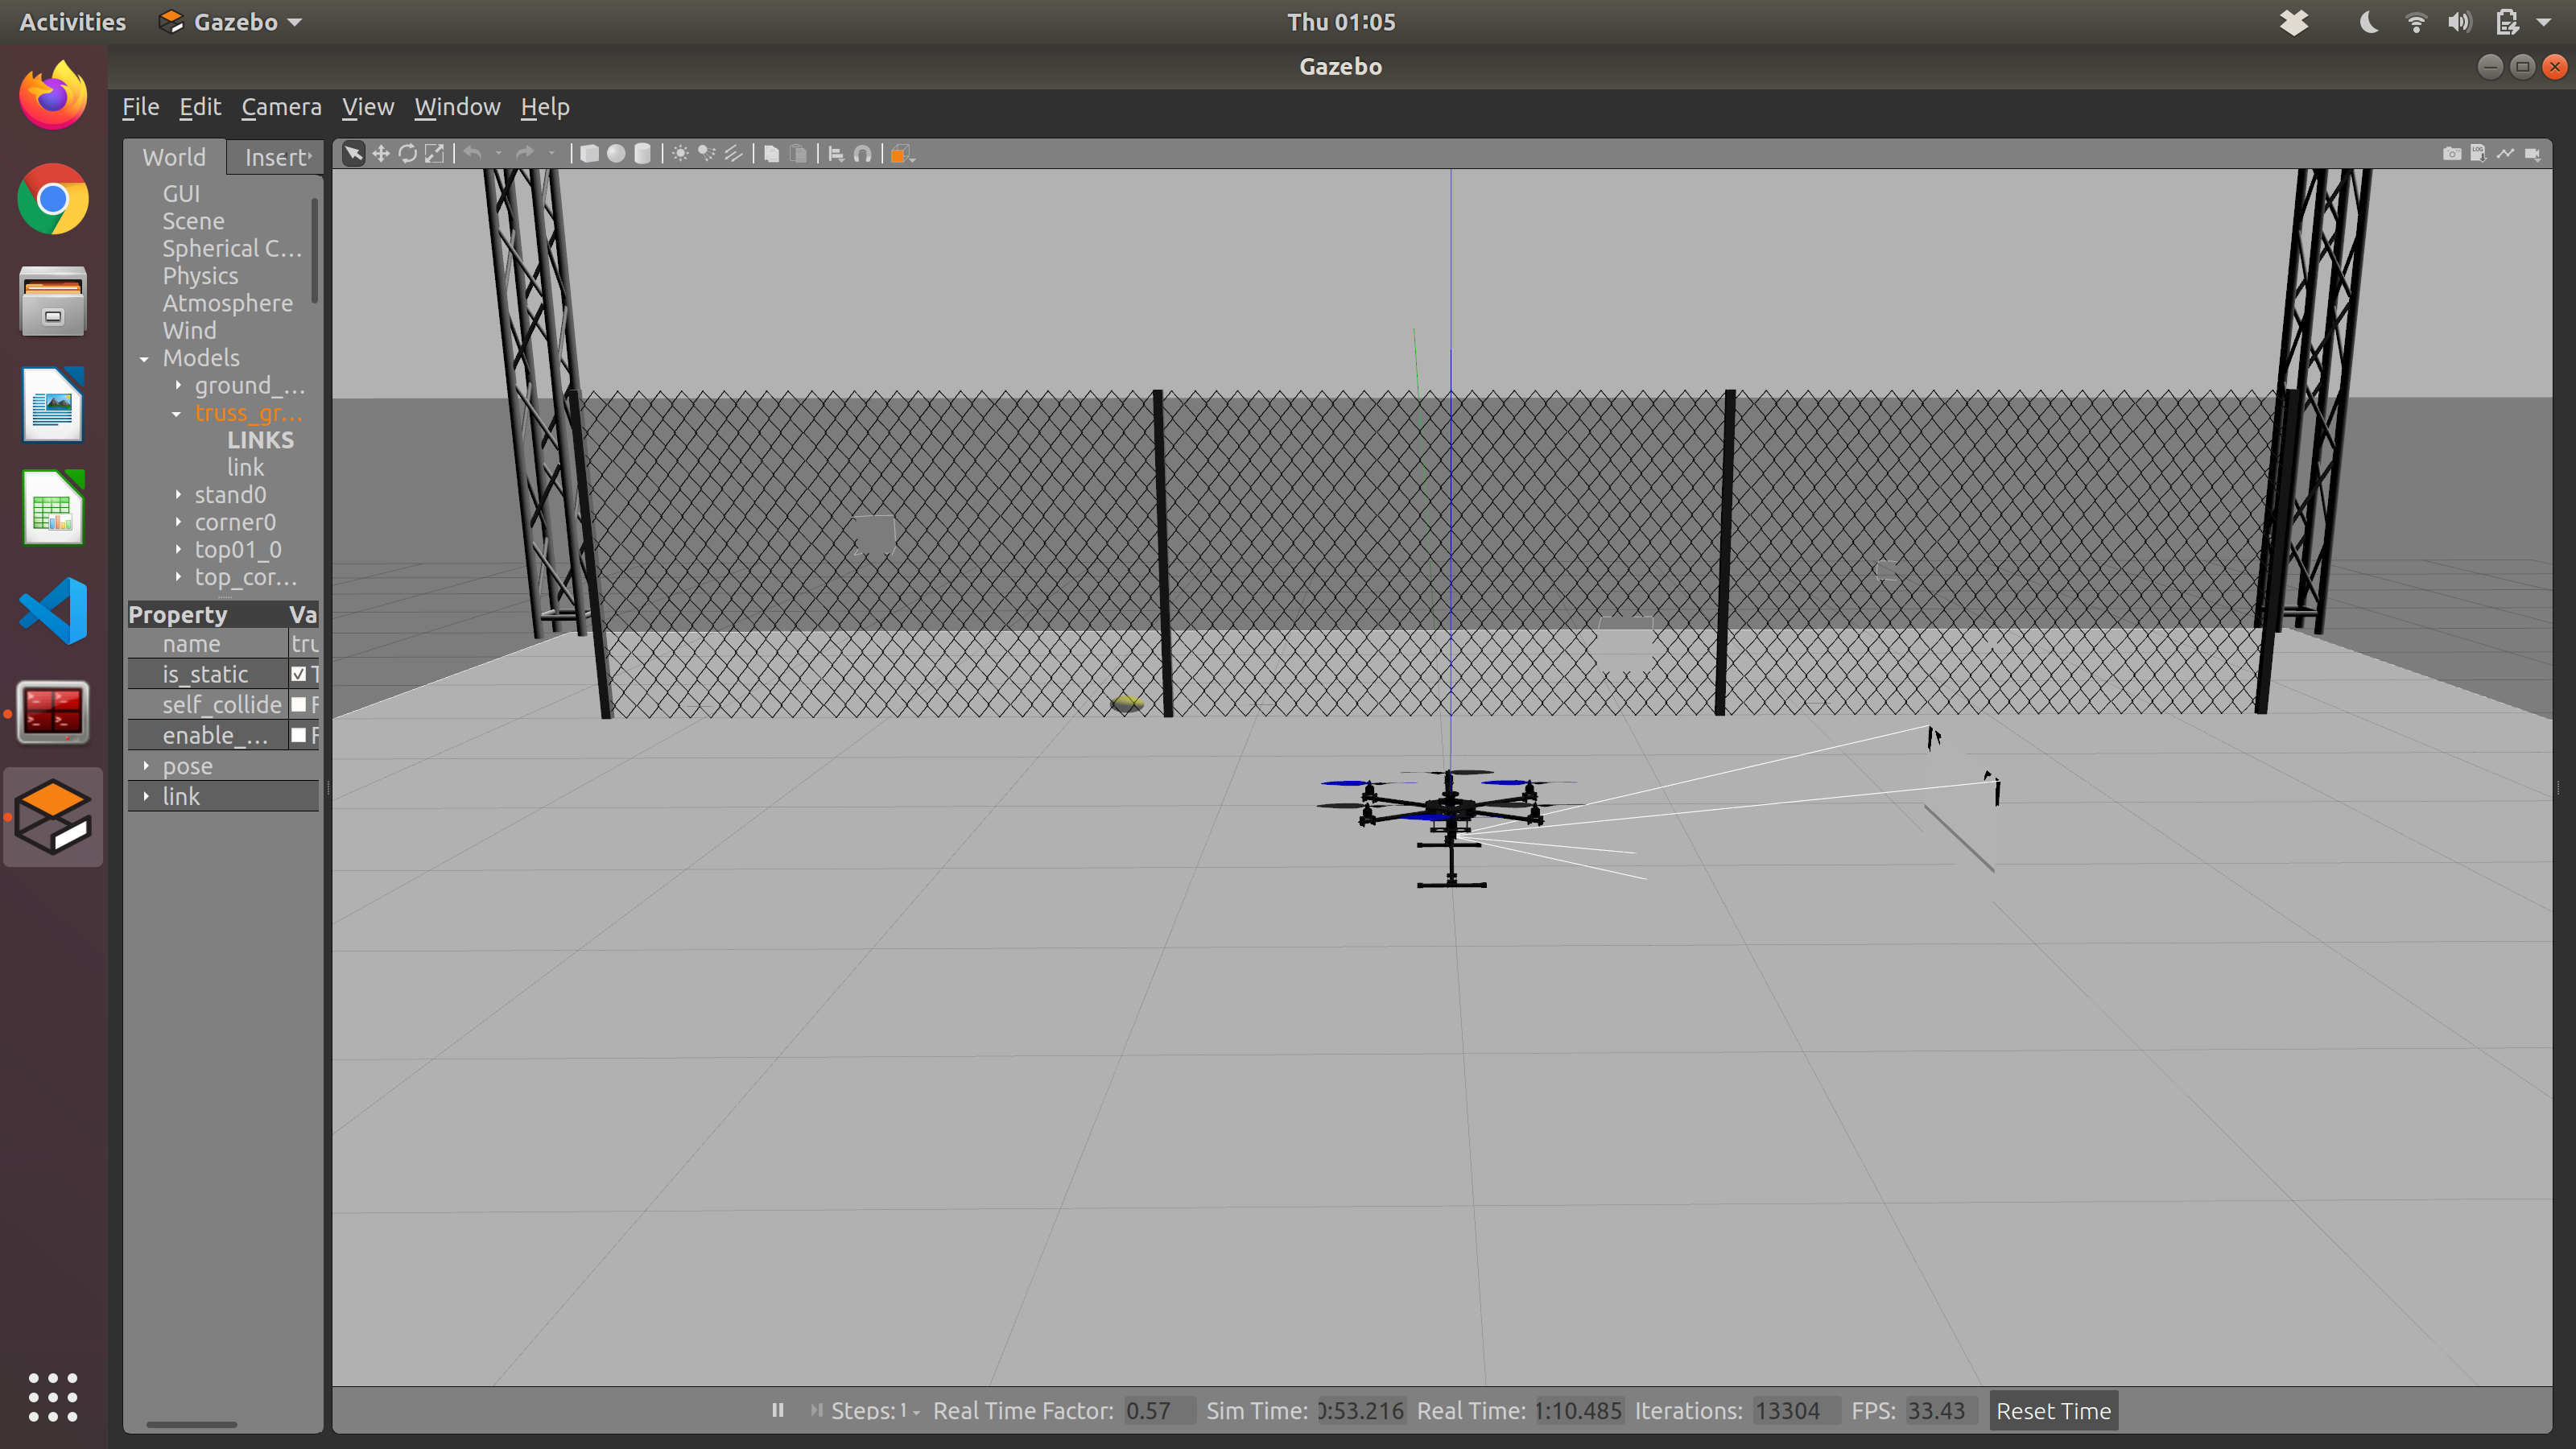
\includegraphics[width=\textwidth]{../Figures/simulation/Simulation_00.png}
        \end{subfigure}
        \begin{subfigure}{\figSize}
            \centering
            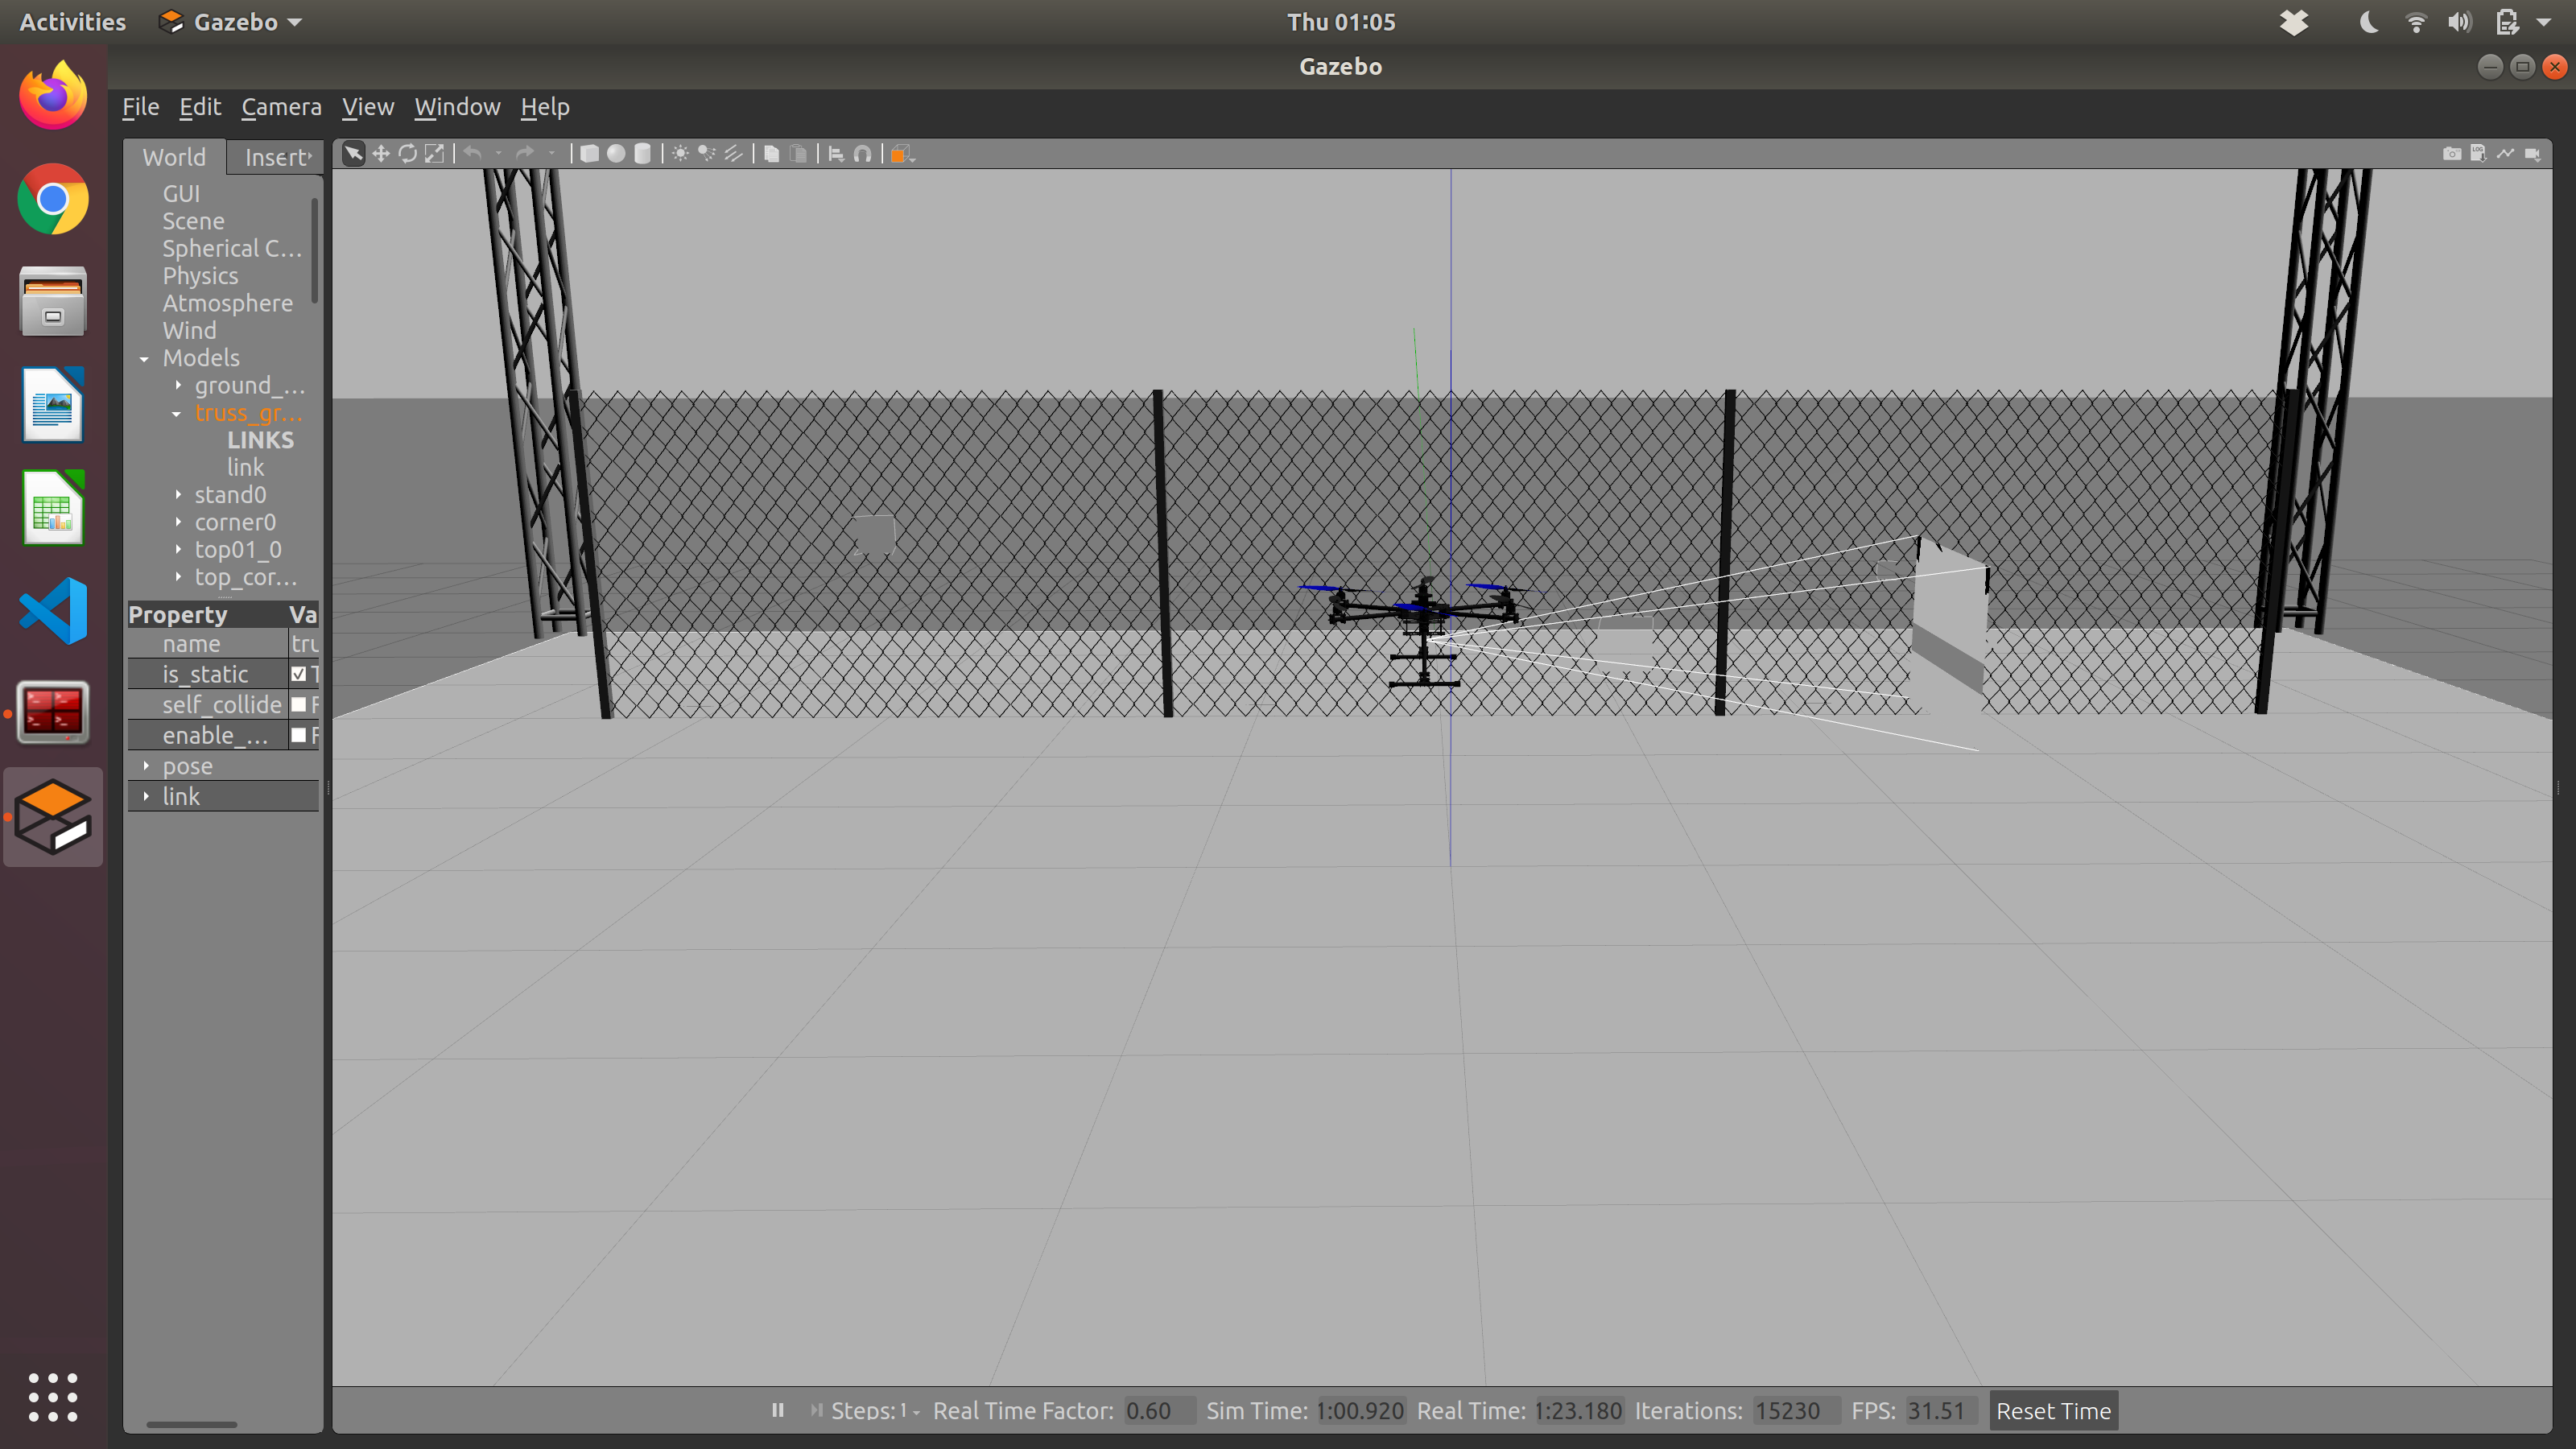
\includegraphics[width=\textwidth]{../Figures/simulation/Simulation_01.png}
        \end{subfigure}
        \begin{subfigure}{\figSize}
            \centering
            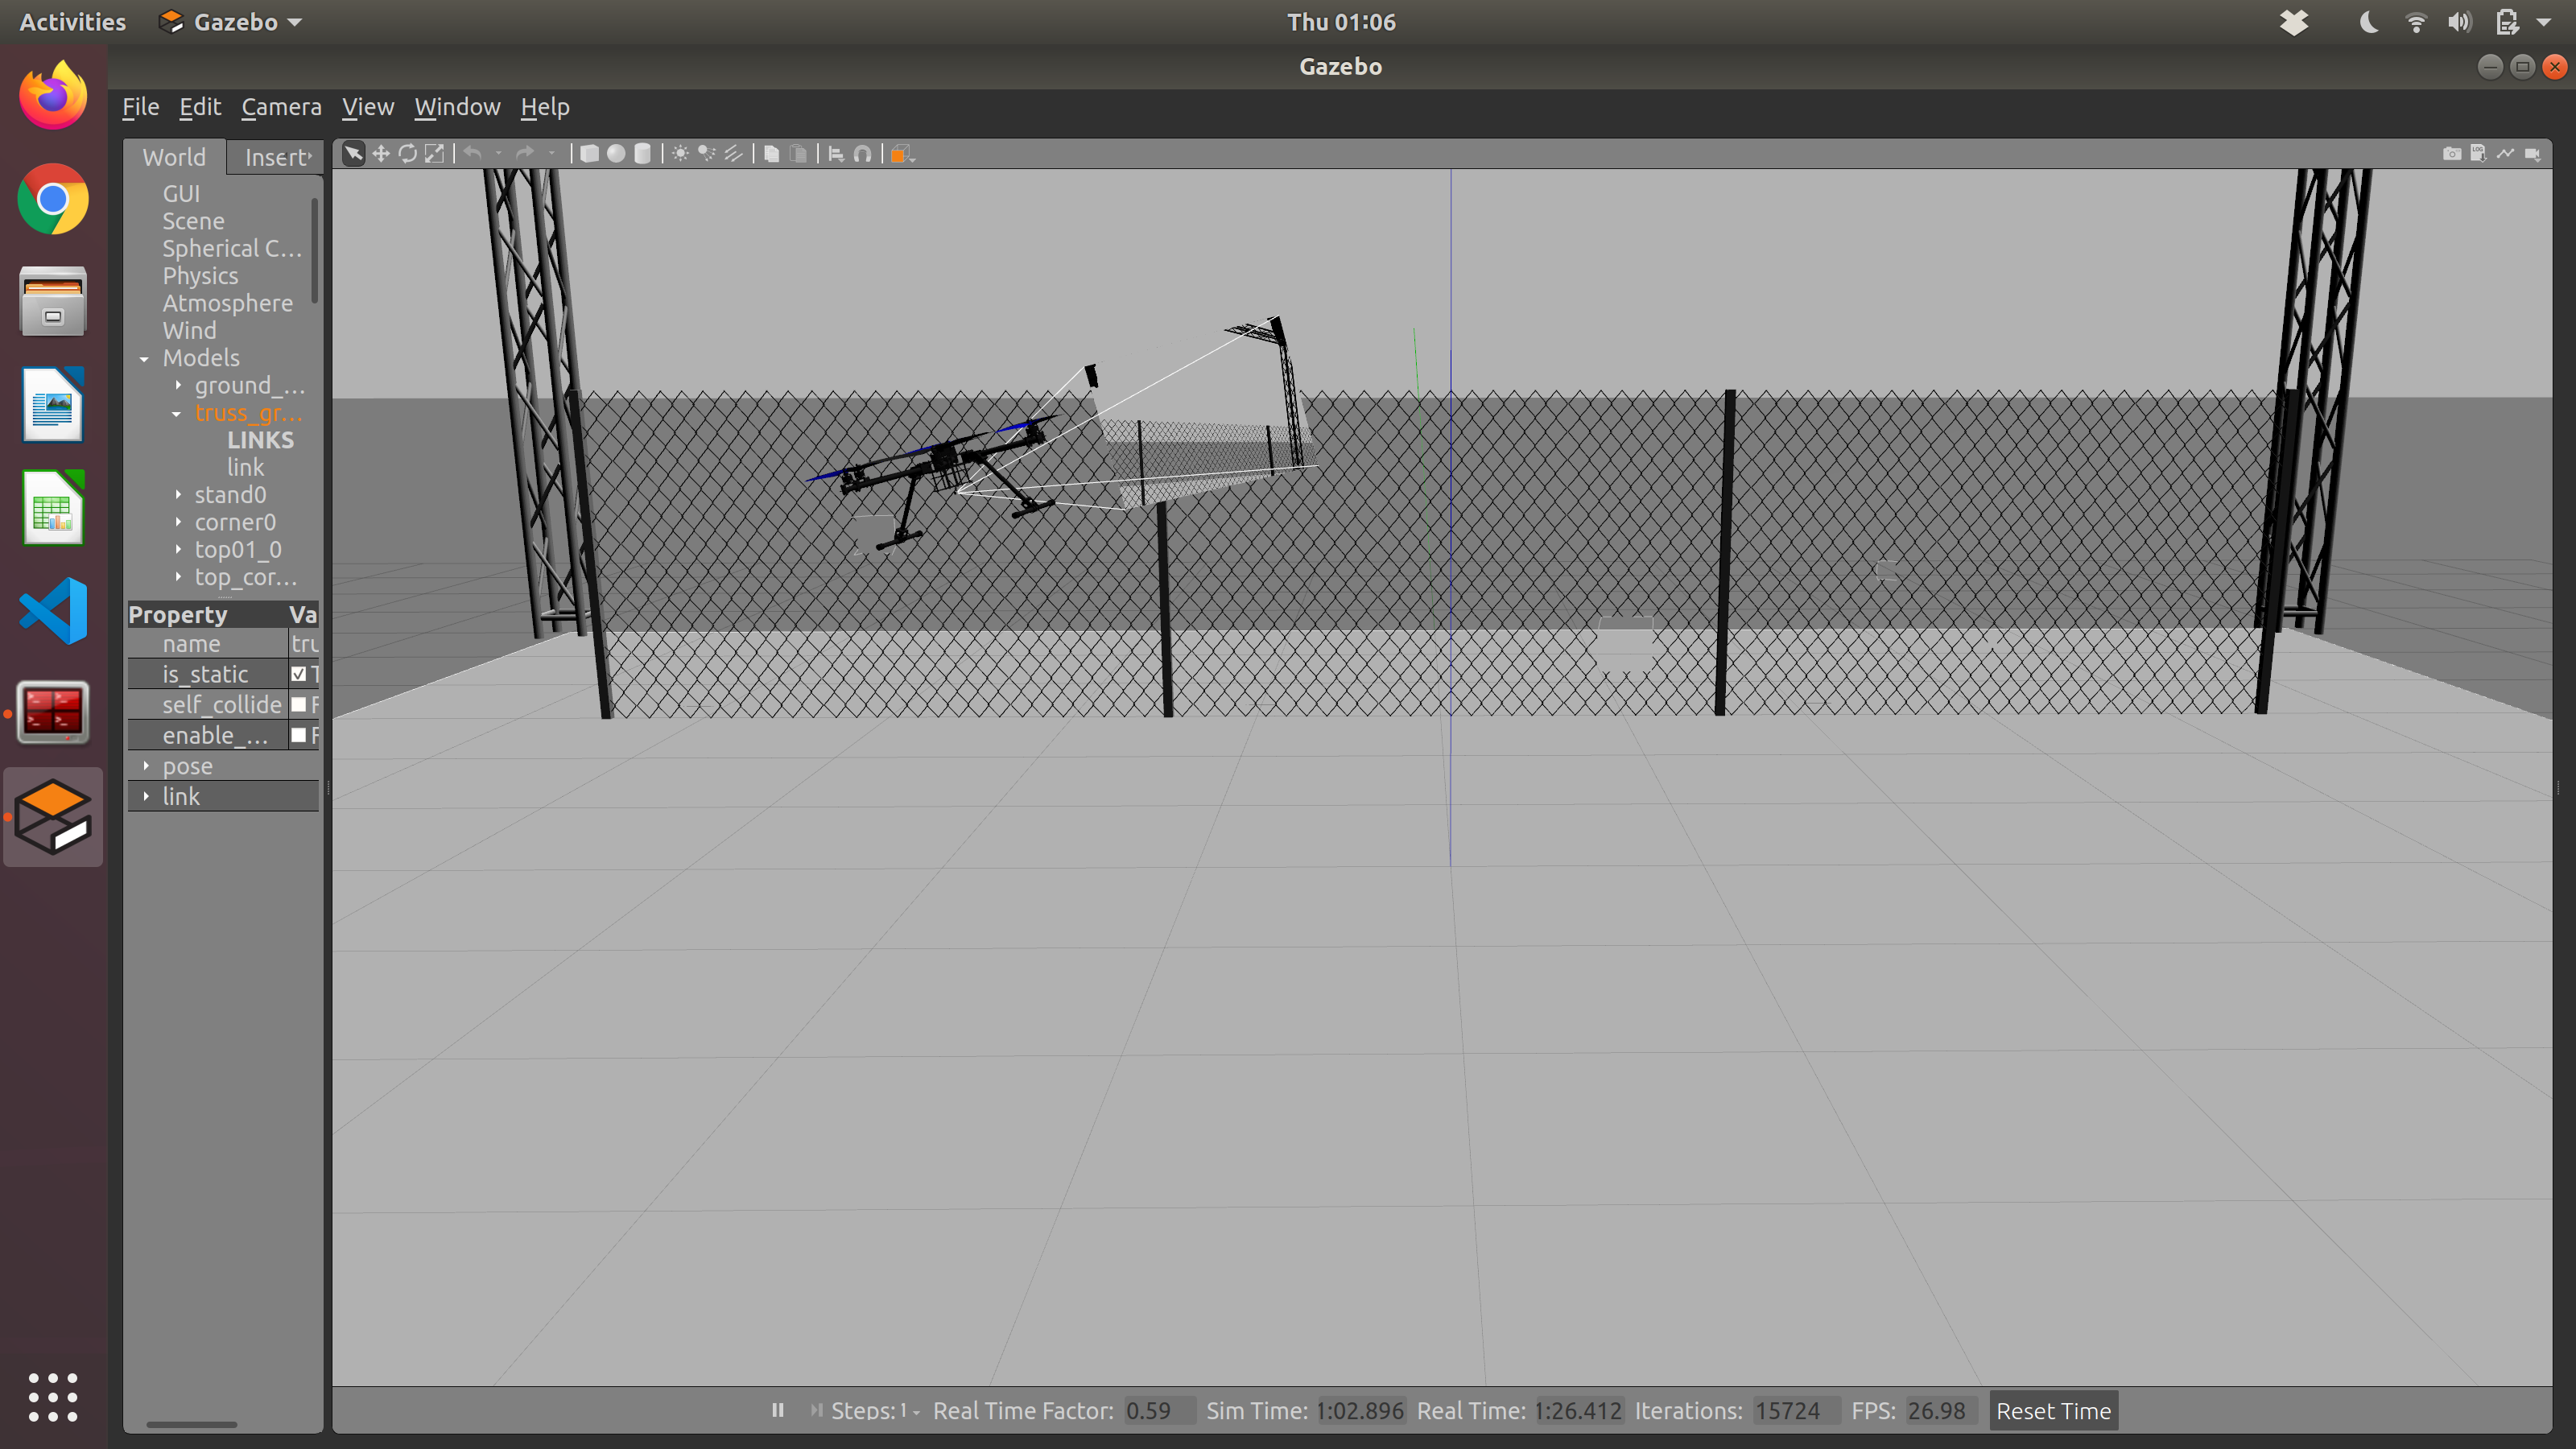
\includegraphics[width=\textwidth]{../Figures/simulation/Simulation_02.png}
        \end{subfigure}
        \begin{subfigure}{\figSize}
            \centering
            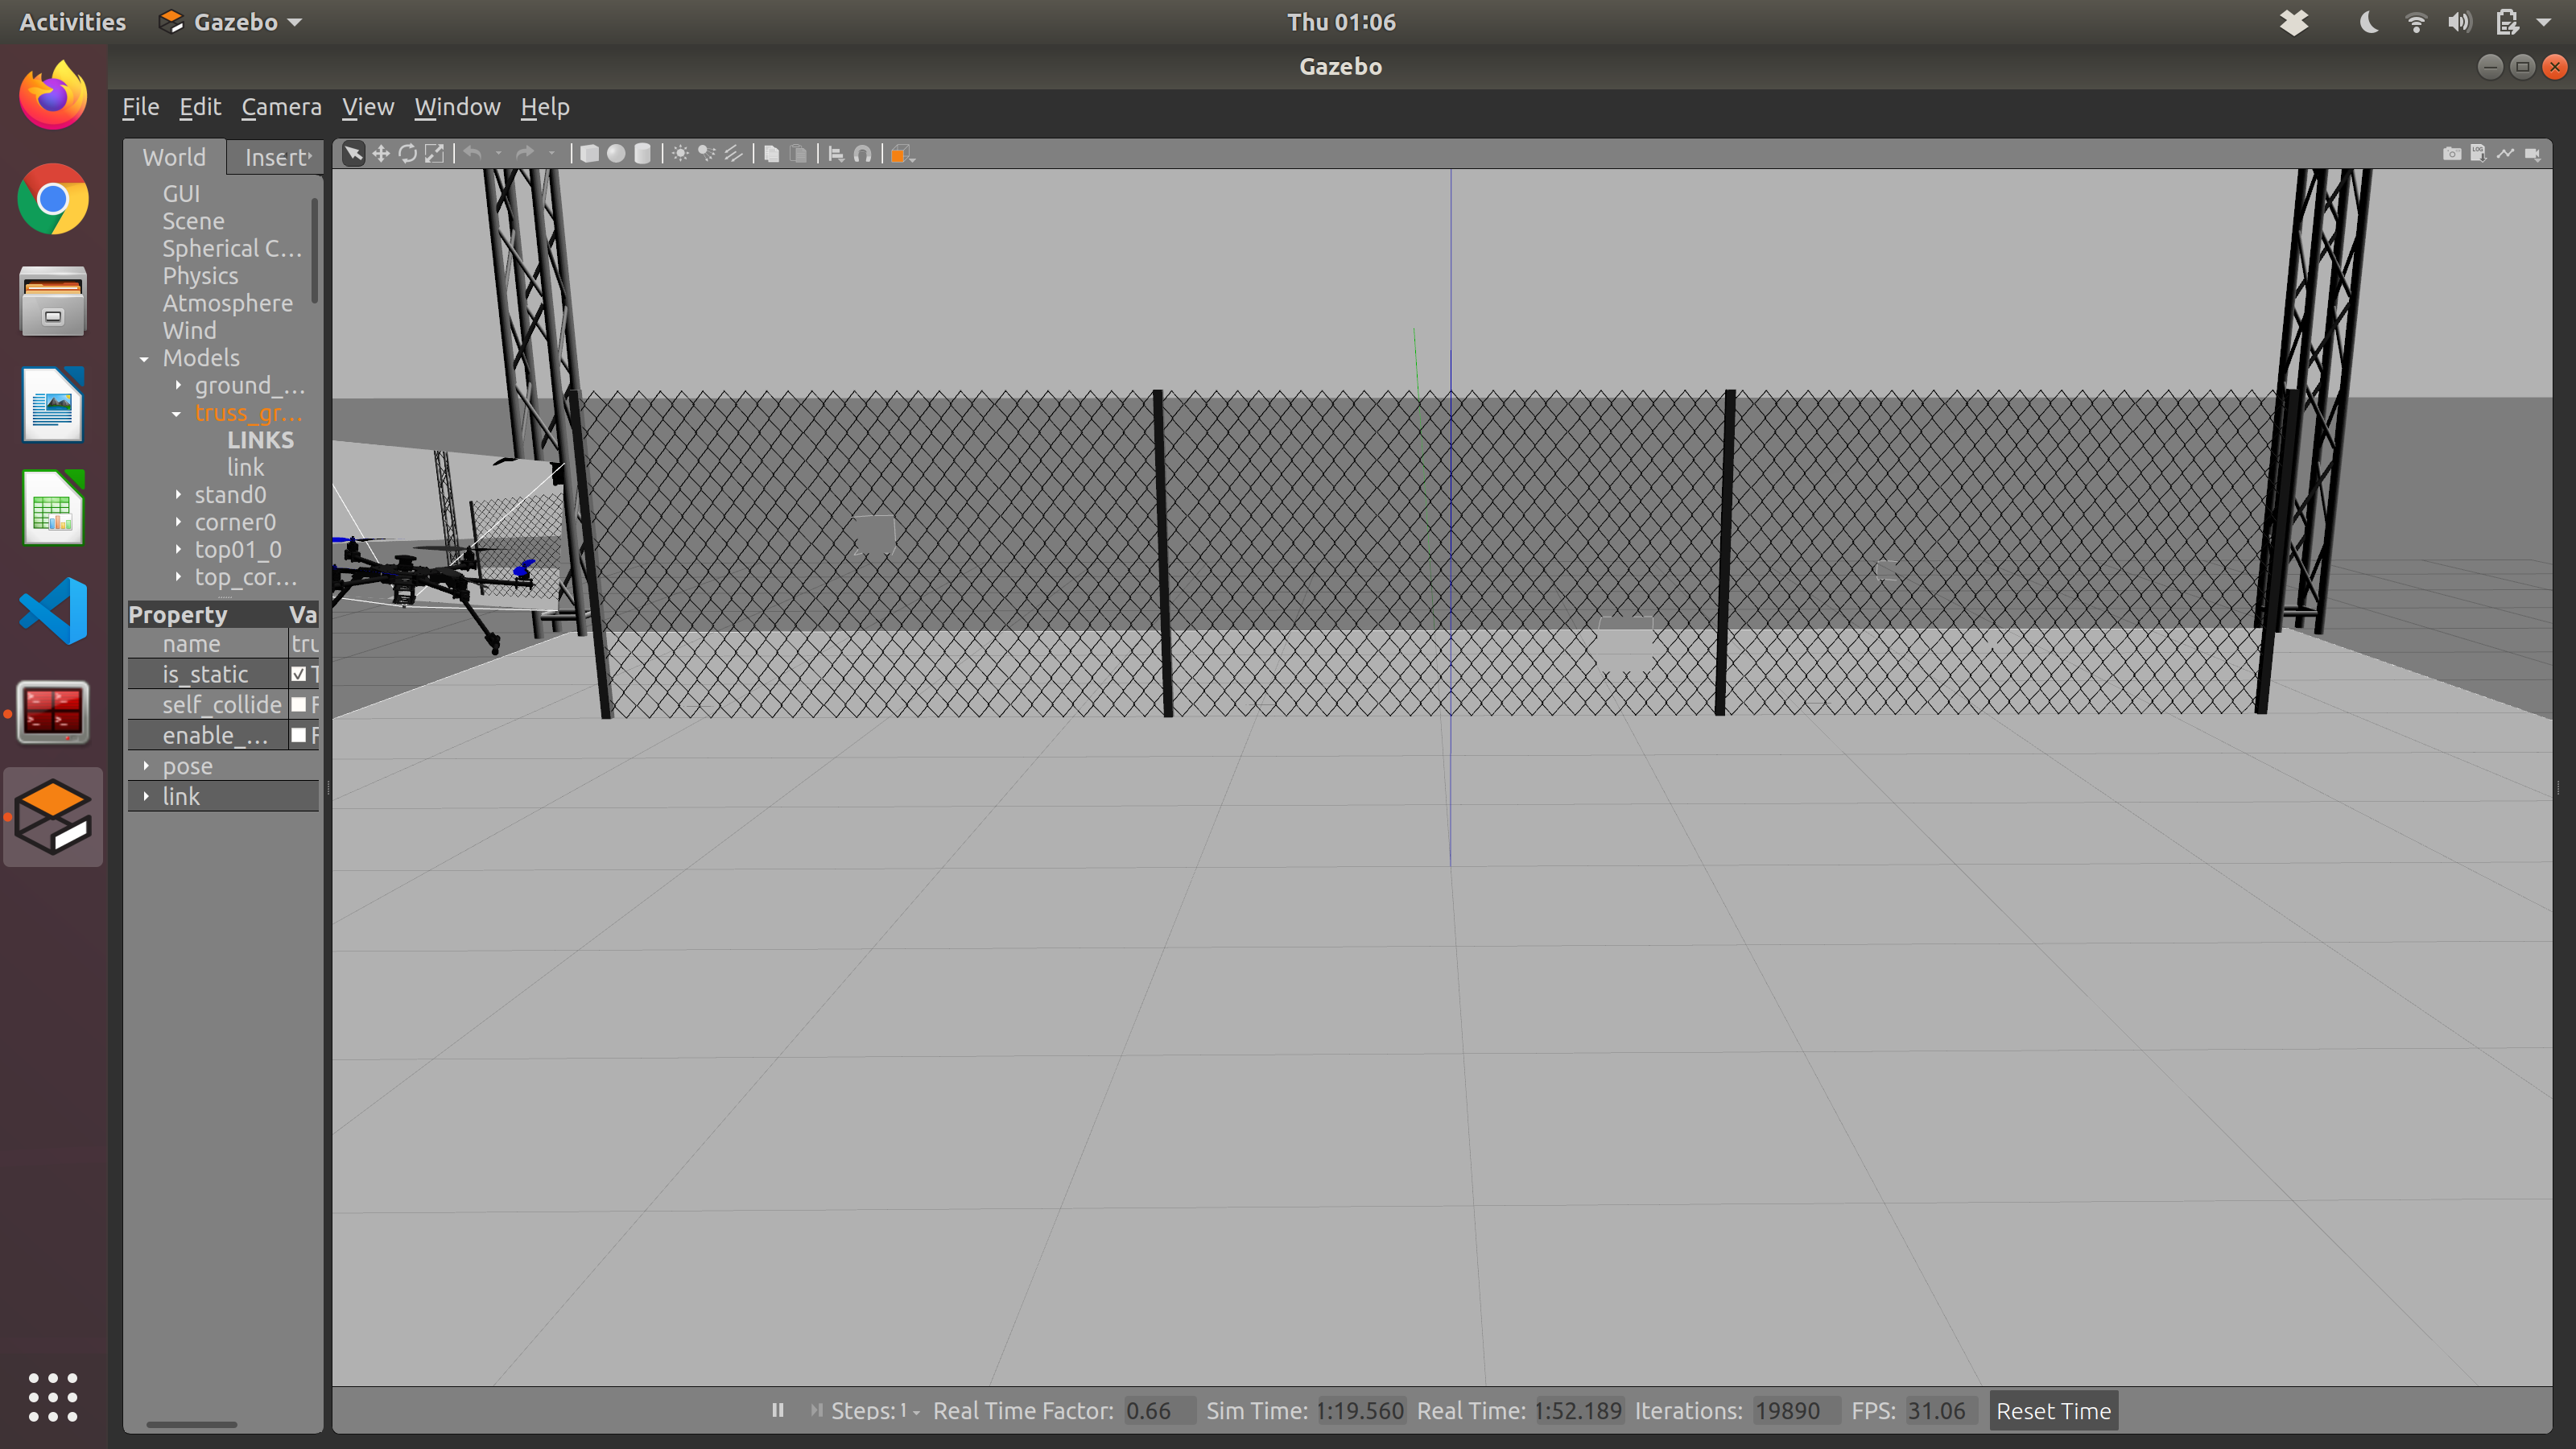
\includegraphics[width=\textwidth]{../Figures/simulation/Simulation_03.png}
        \end{subfigure}
        \begin{subfigure}{\figSize}
            \centering
            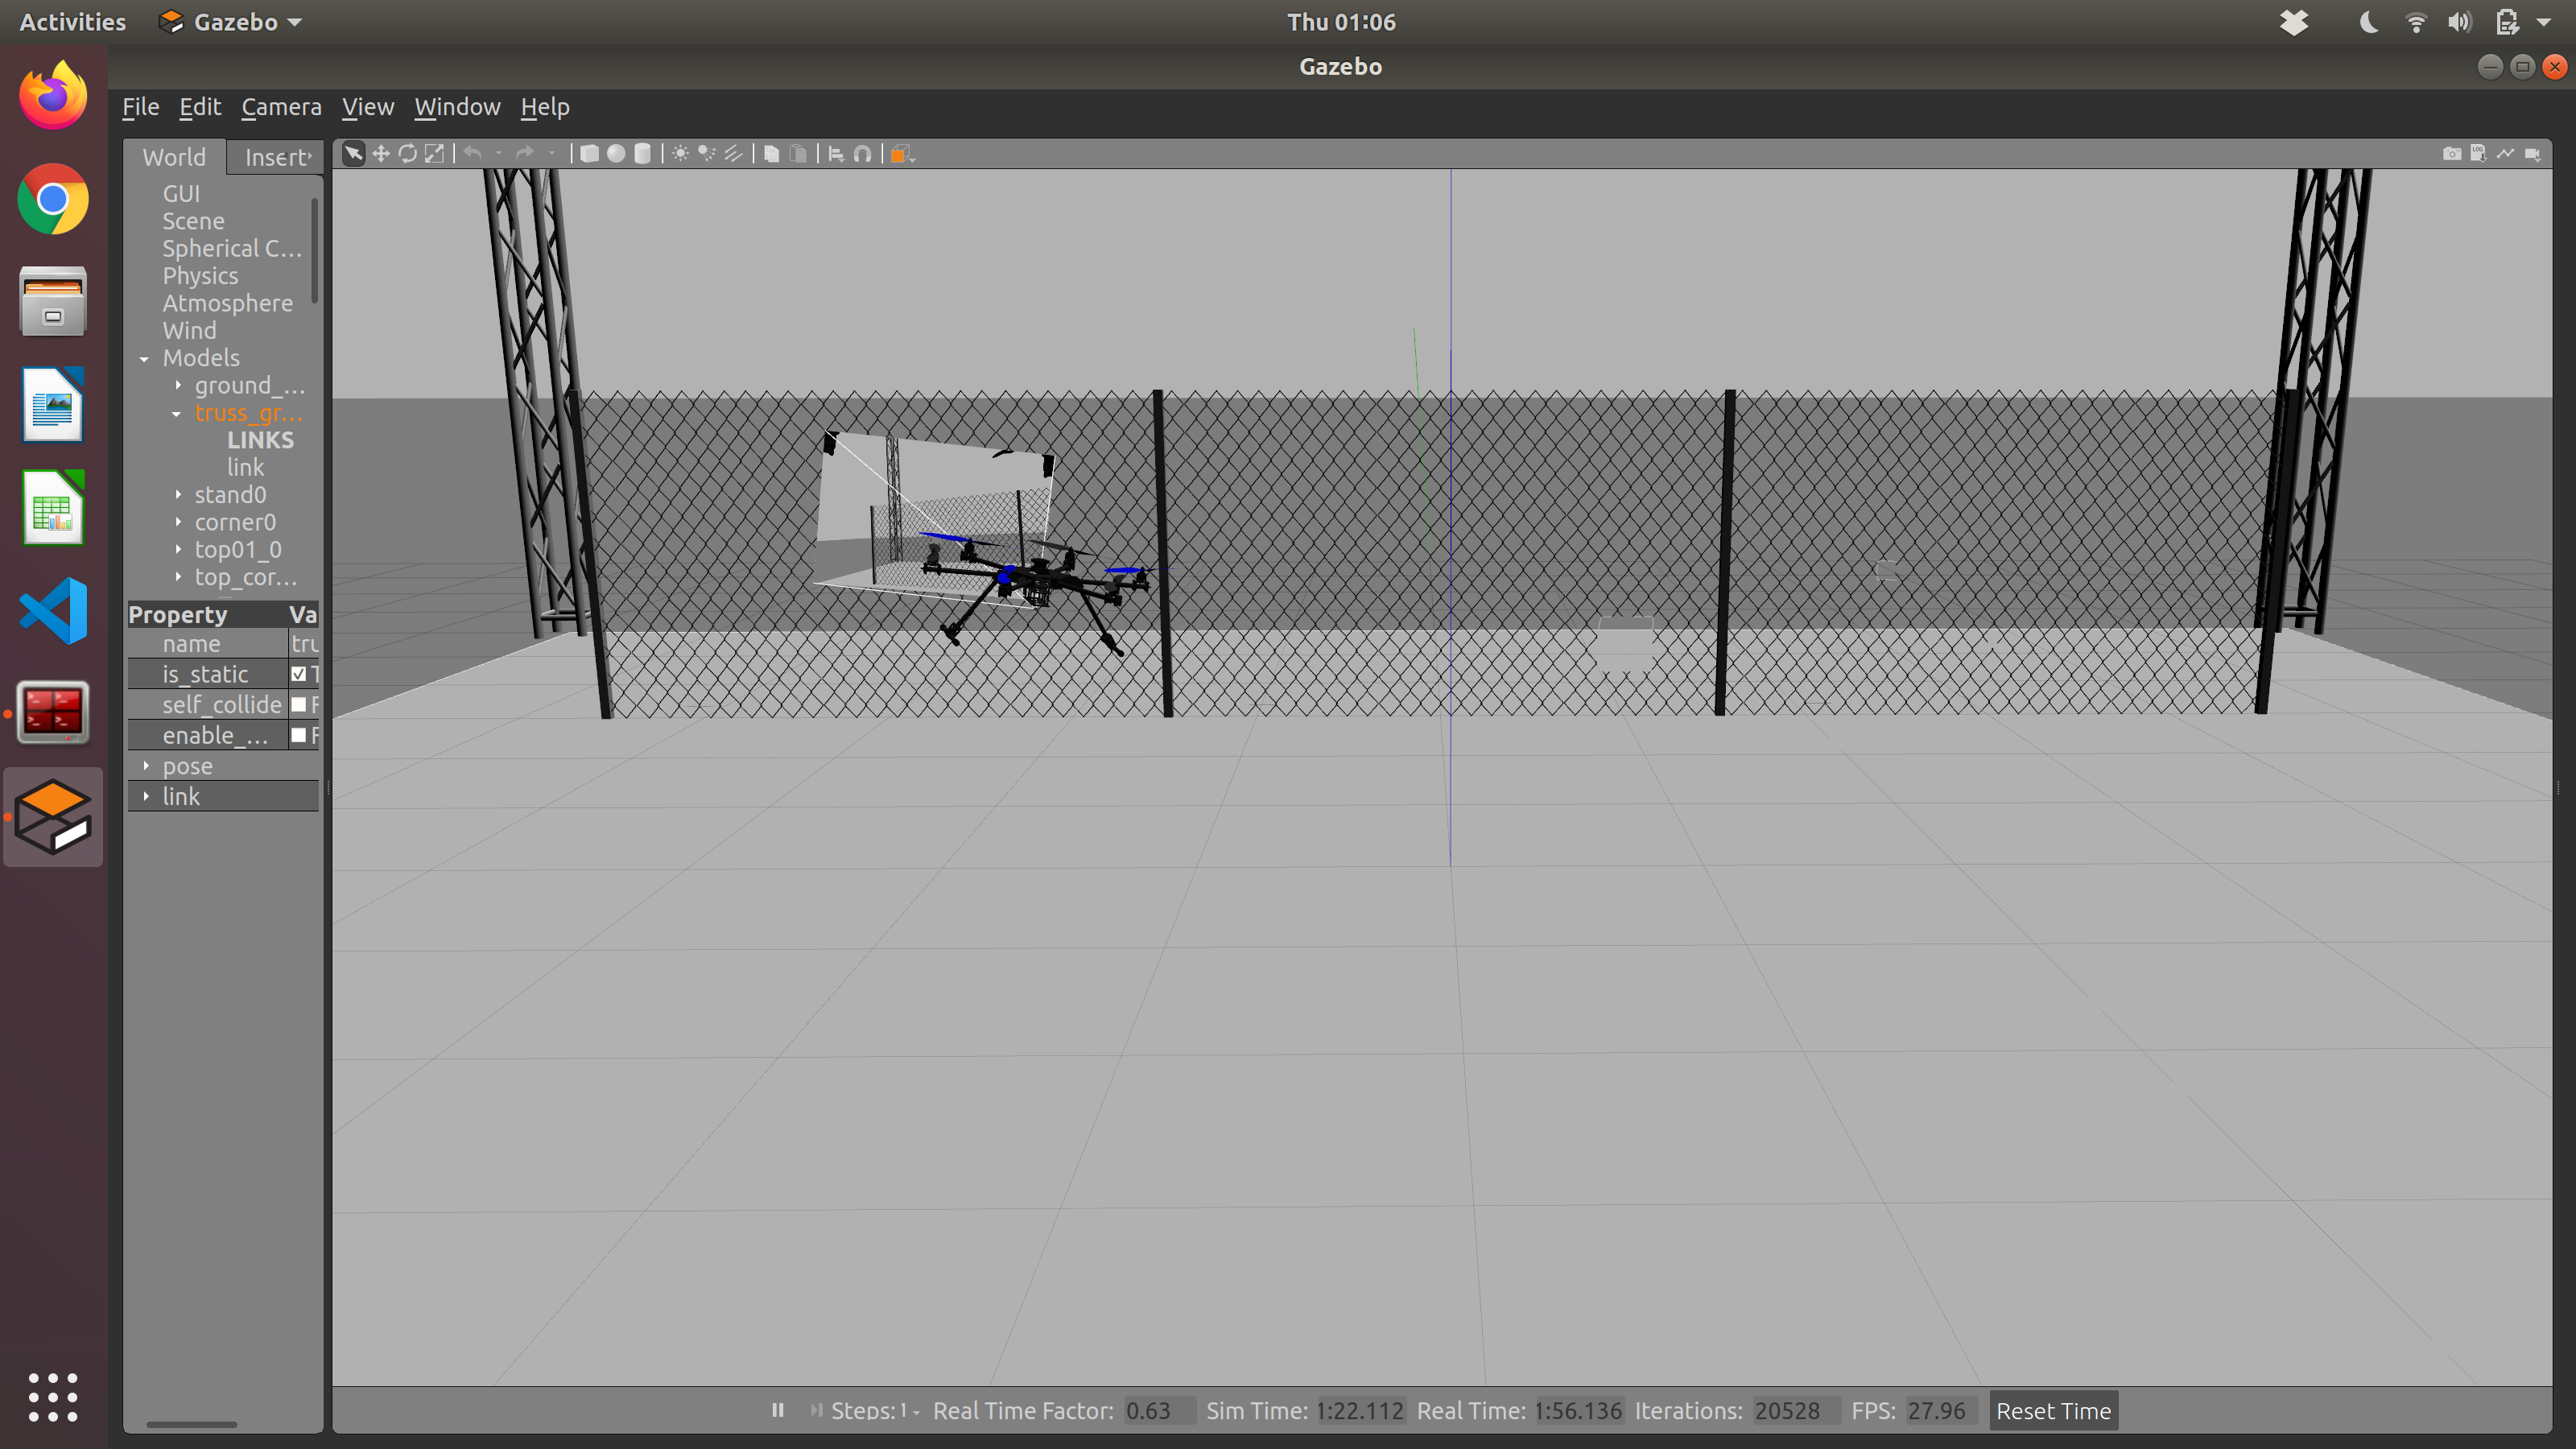
\includegraphics[width=\textwidth]{../Figures/simulation/Simulation_04.png}
        \end{subfigure}
        \begin{subfigure}{\figSize}
            \centering
            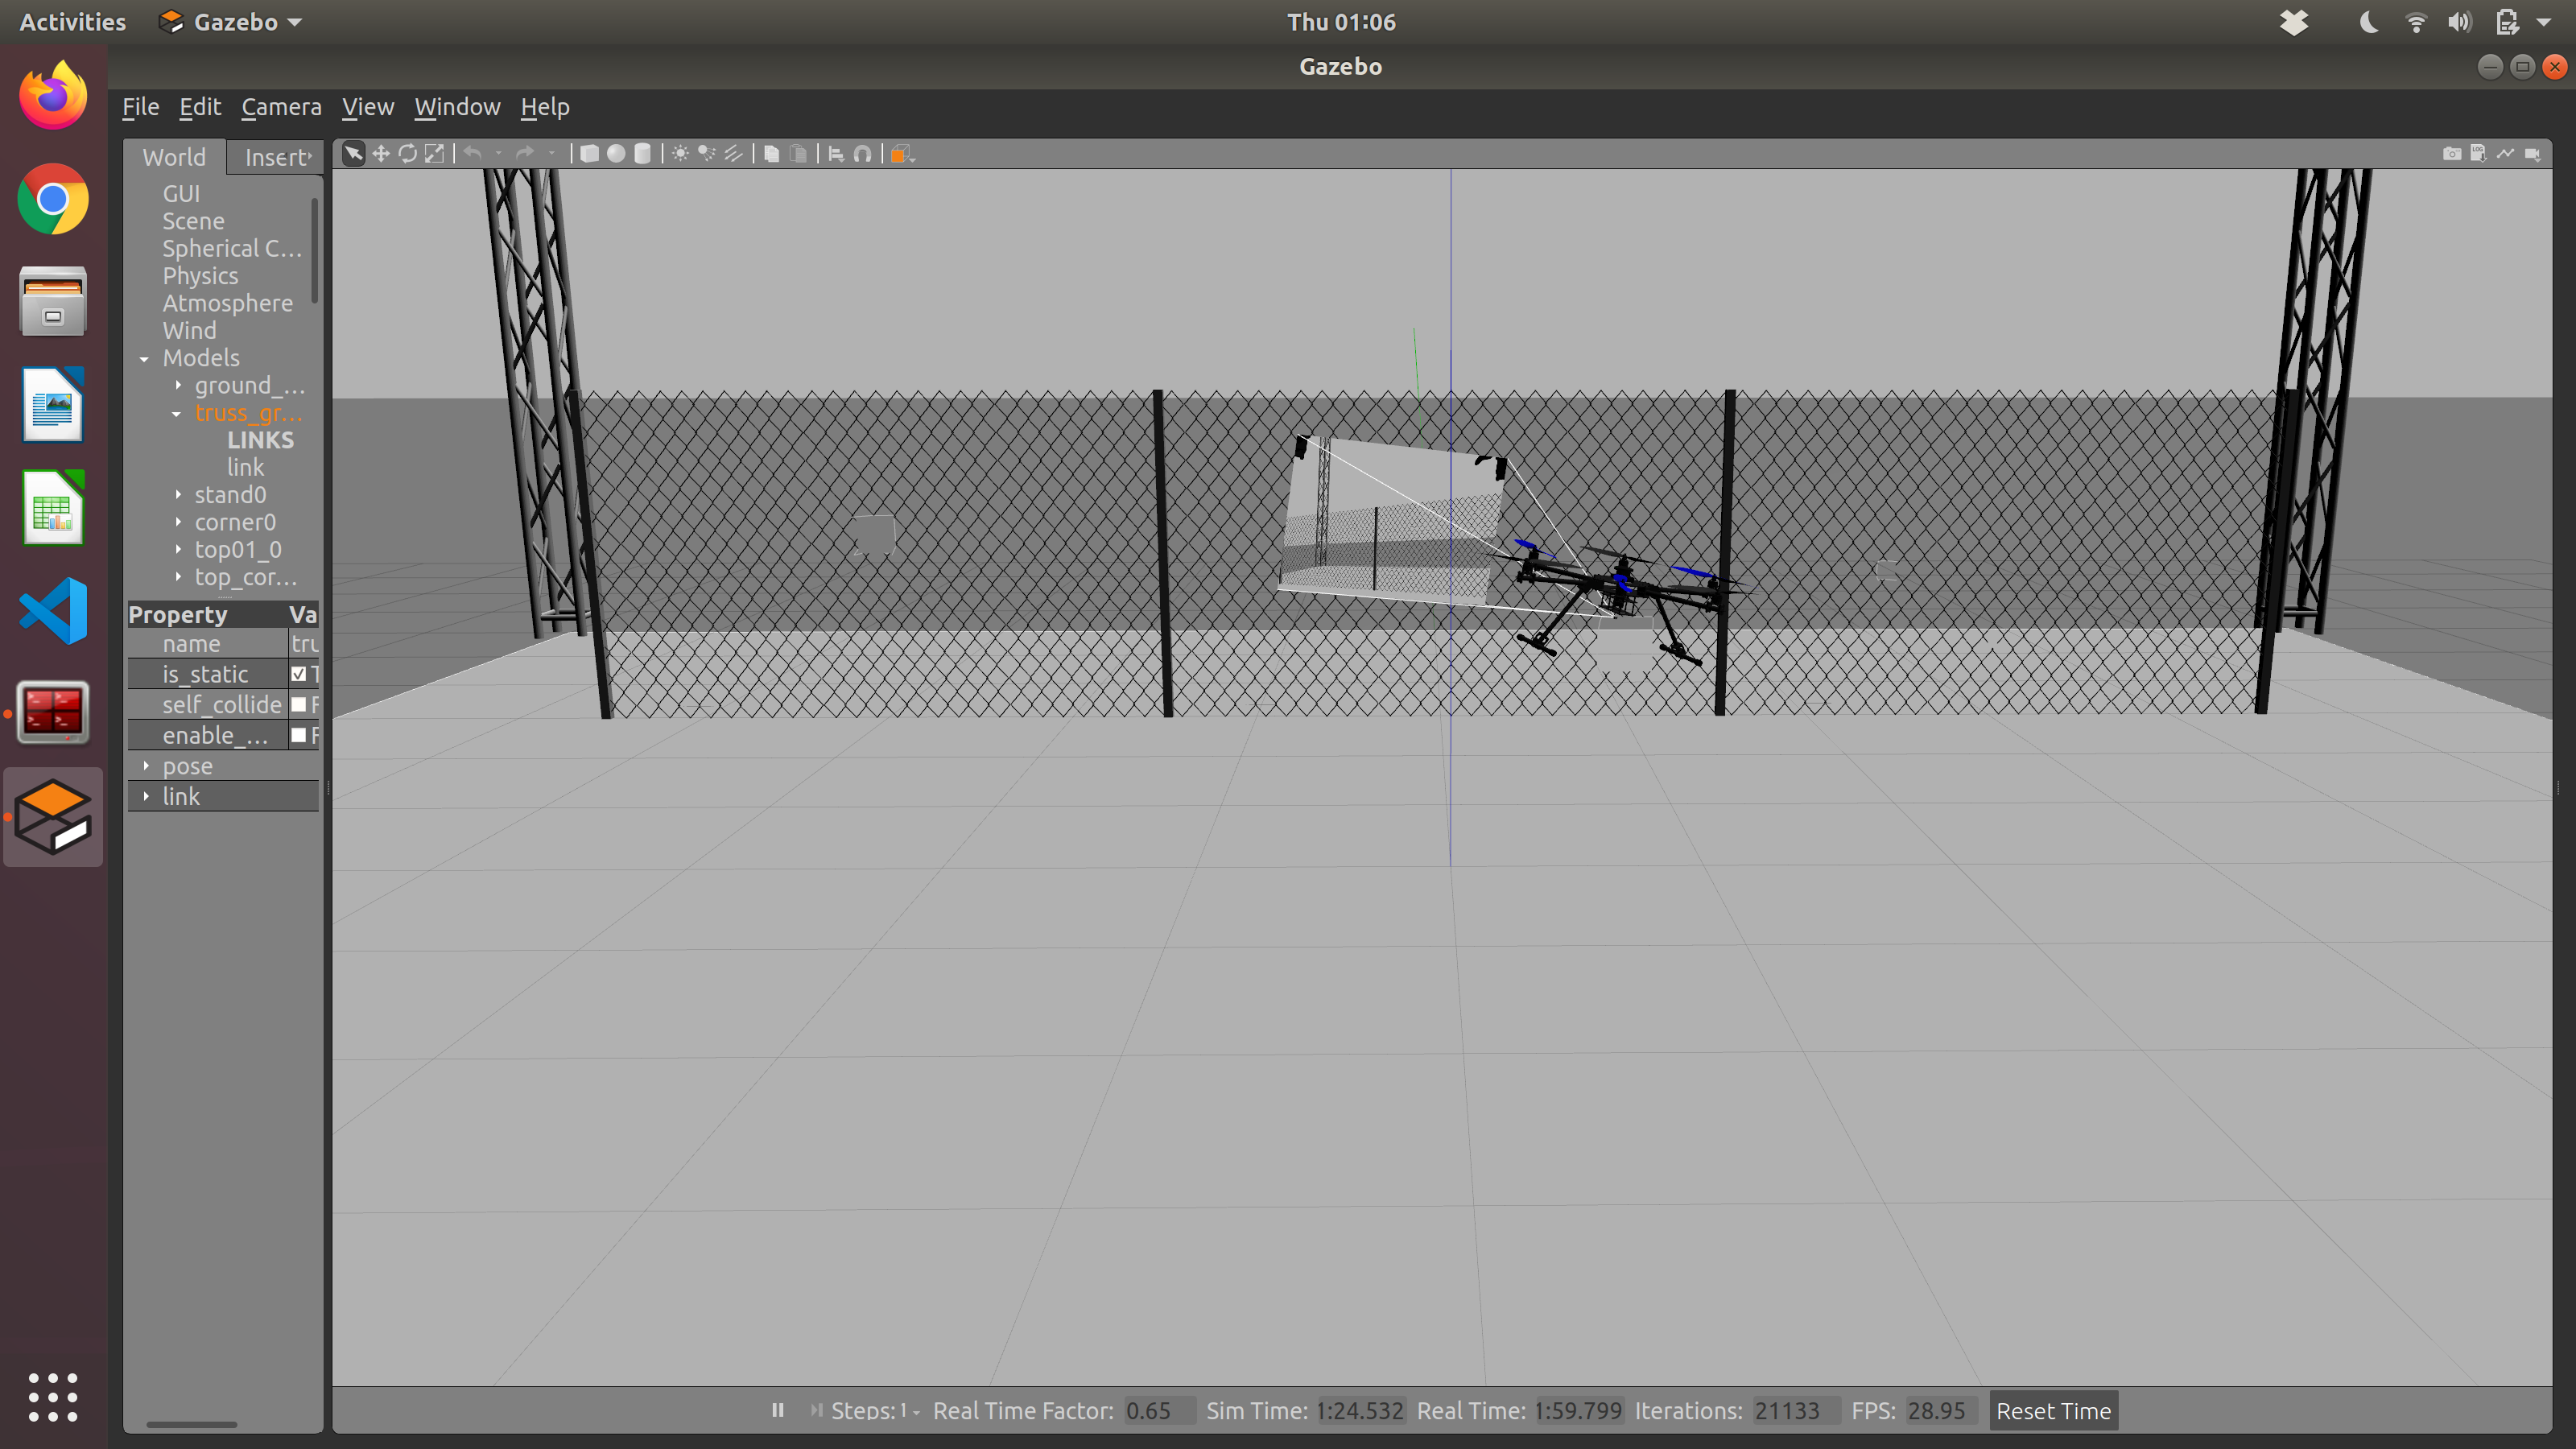
\includegraphics[width=\textwidth]{../Figures/simulation/Simulation_05.png}
        \end{subfigure}
        \begin{subfigure}{\figSize}
            \centering
            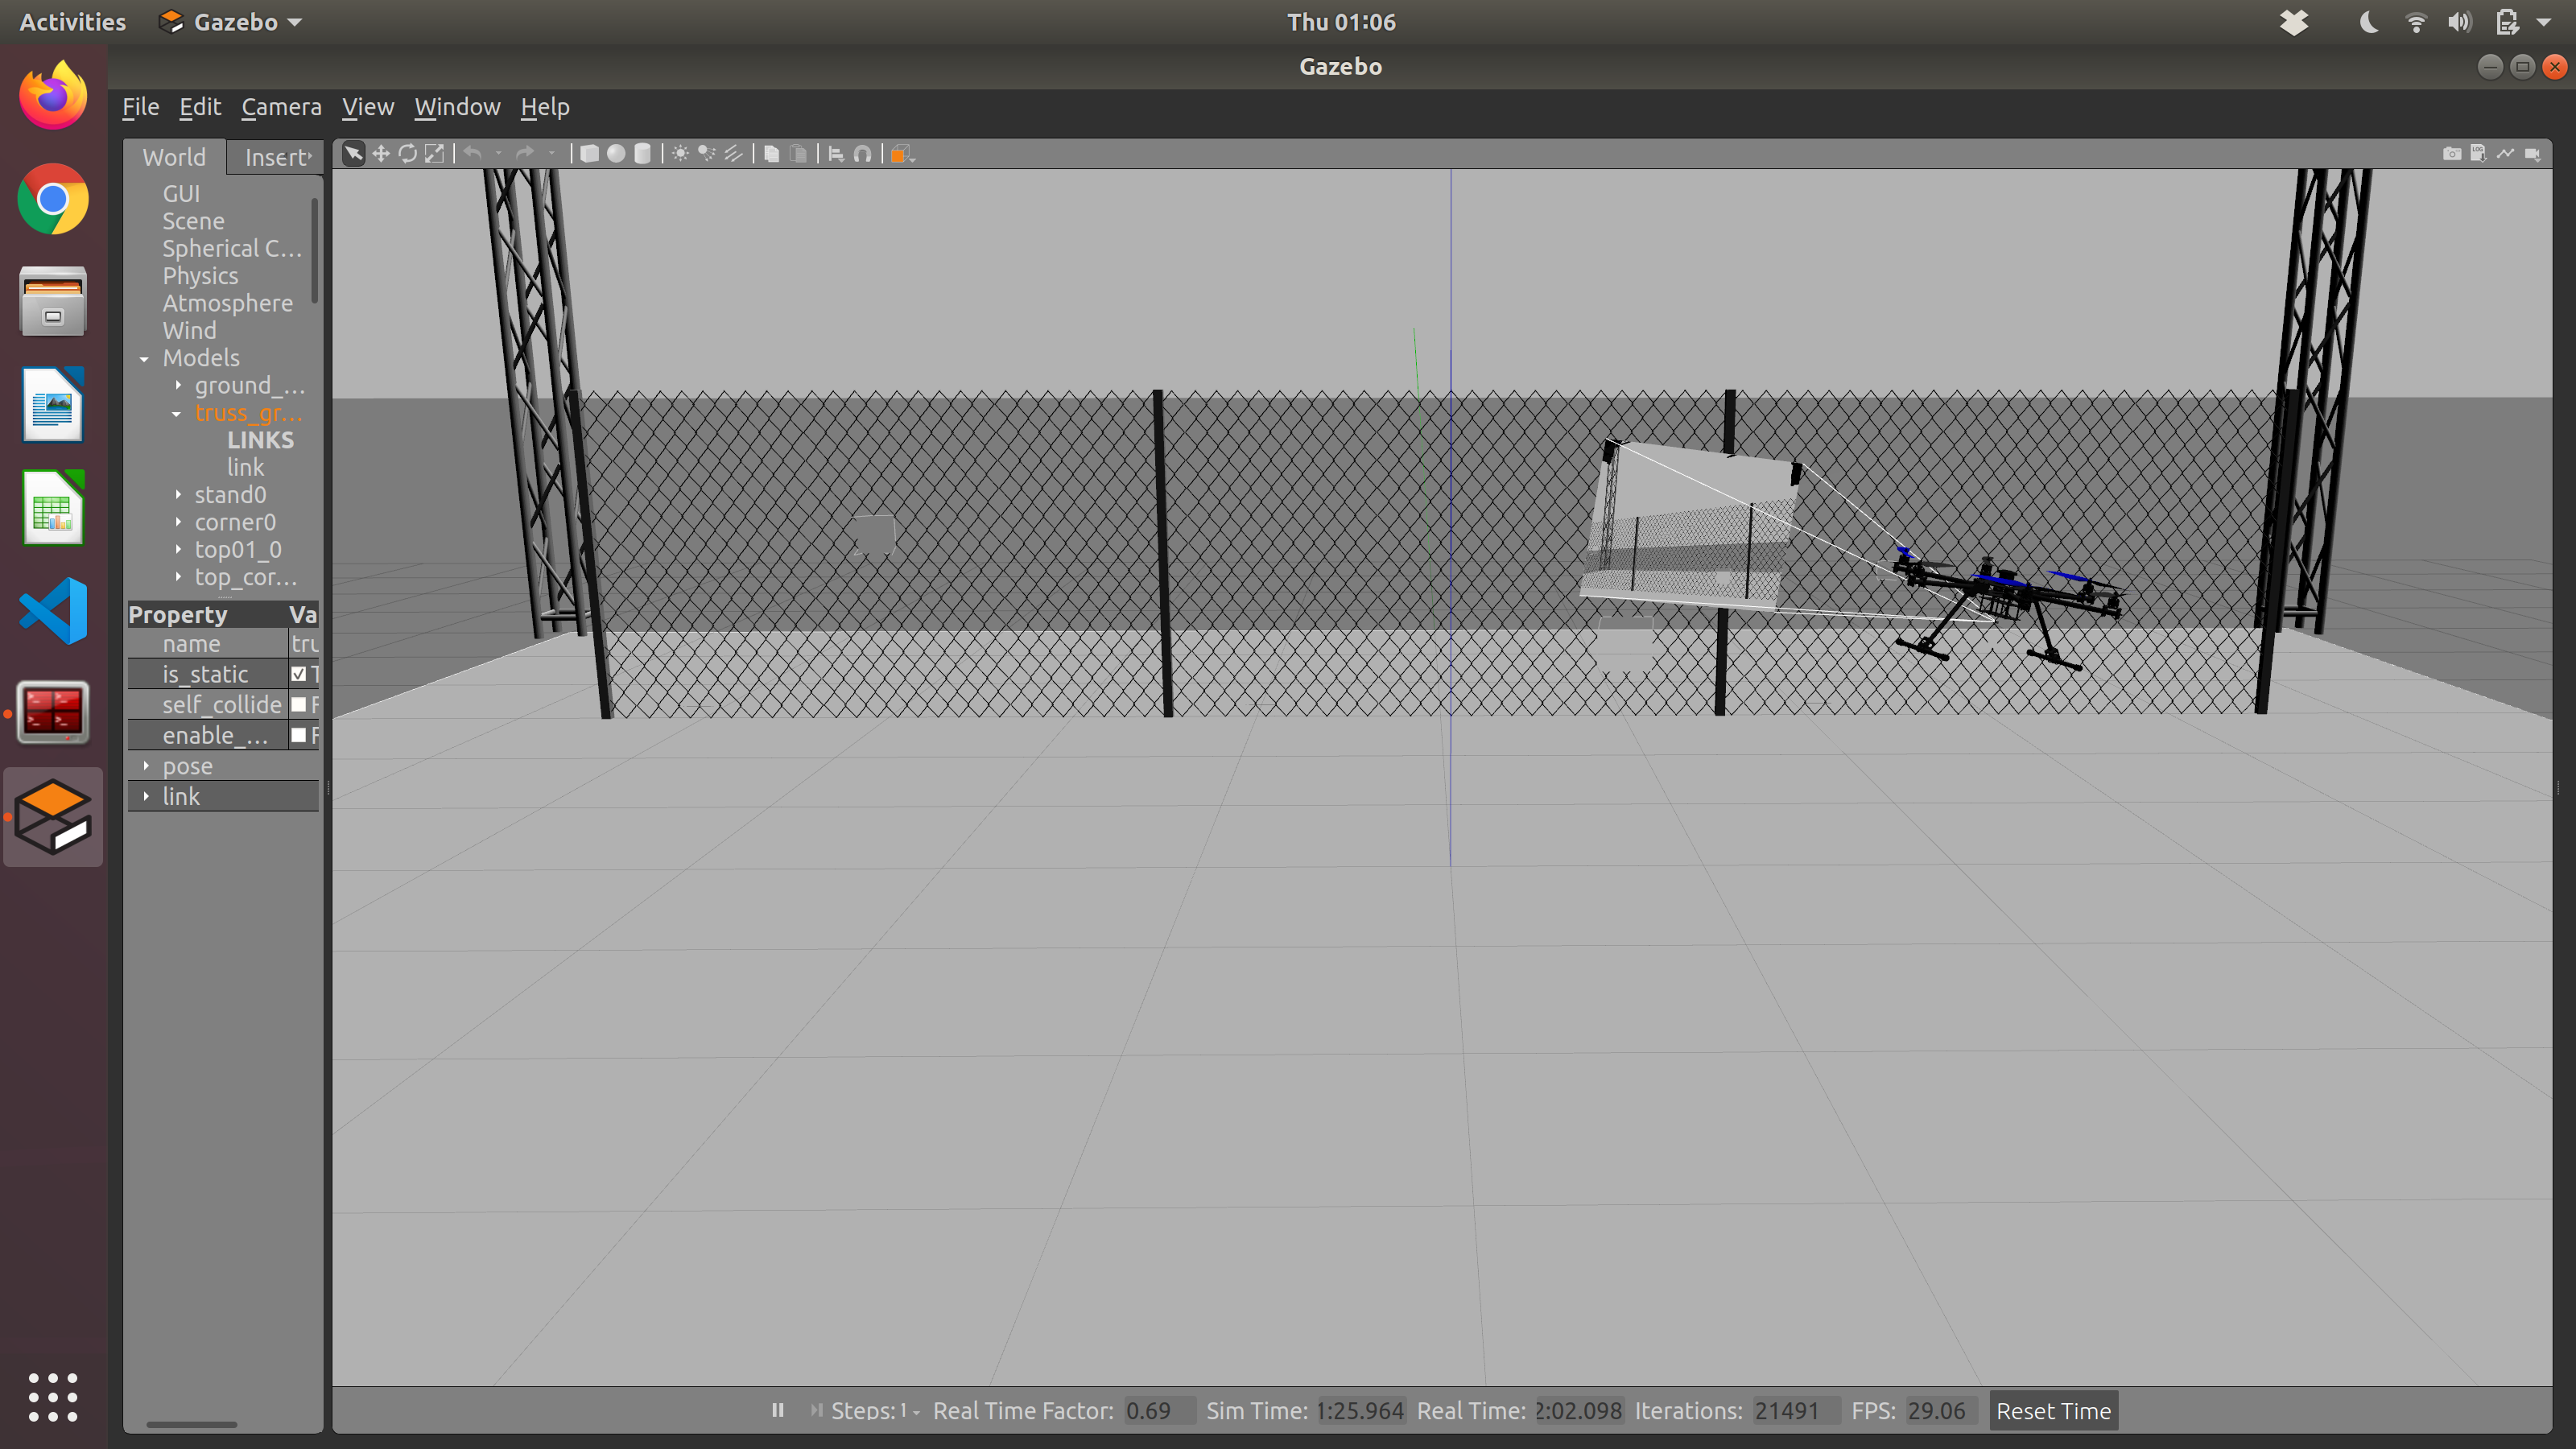
\includegraphics[width=\textwidth]{../Figures/simulation/Simulation_06.png}
        \end{subfigure}
        \begin{subfigure}{\figSize}
            \centering
            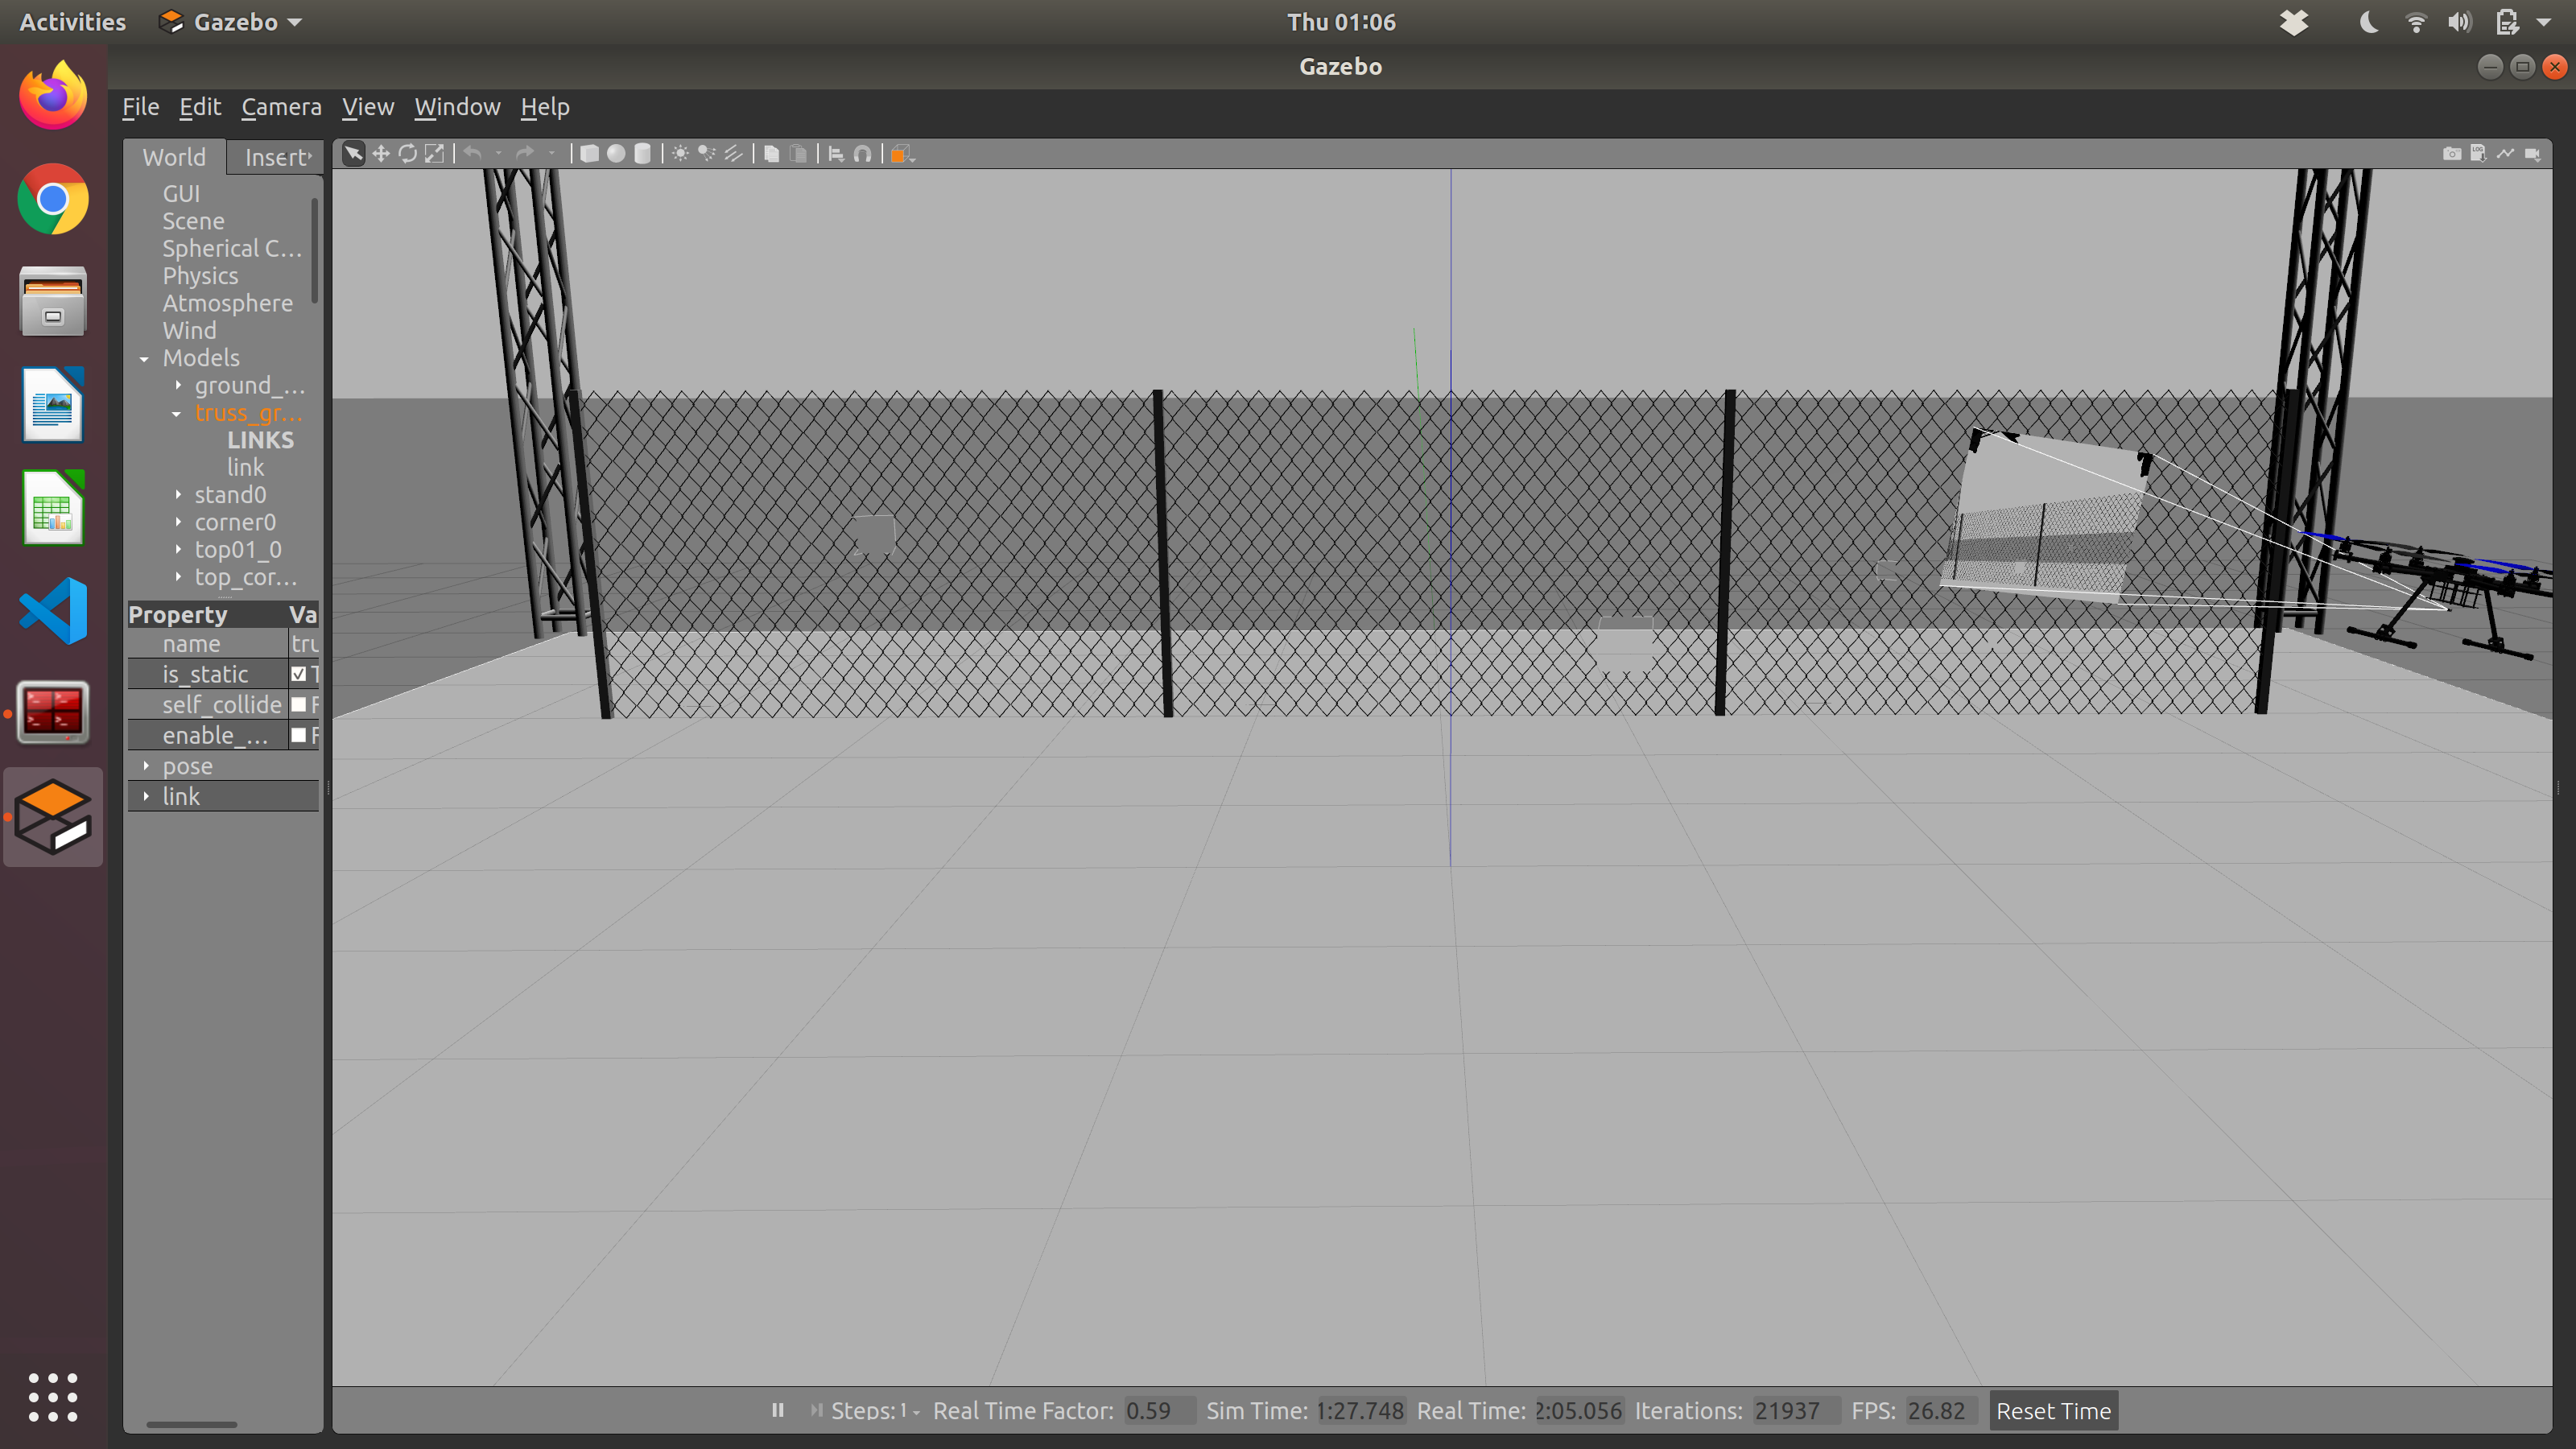
\includegraphics[width=\textwidth]{../Figures/simulation/Simulation_07.png}
        \end{subfigure}
        \begin{subfigure}{\figSize}
            \centering
            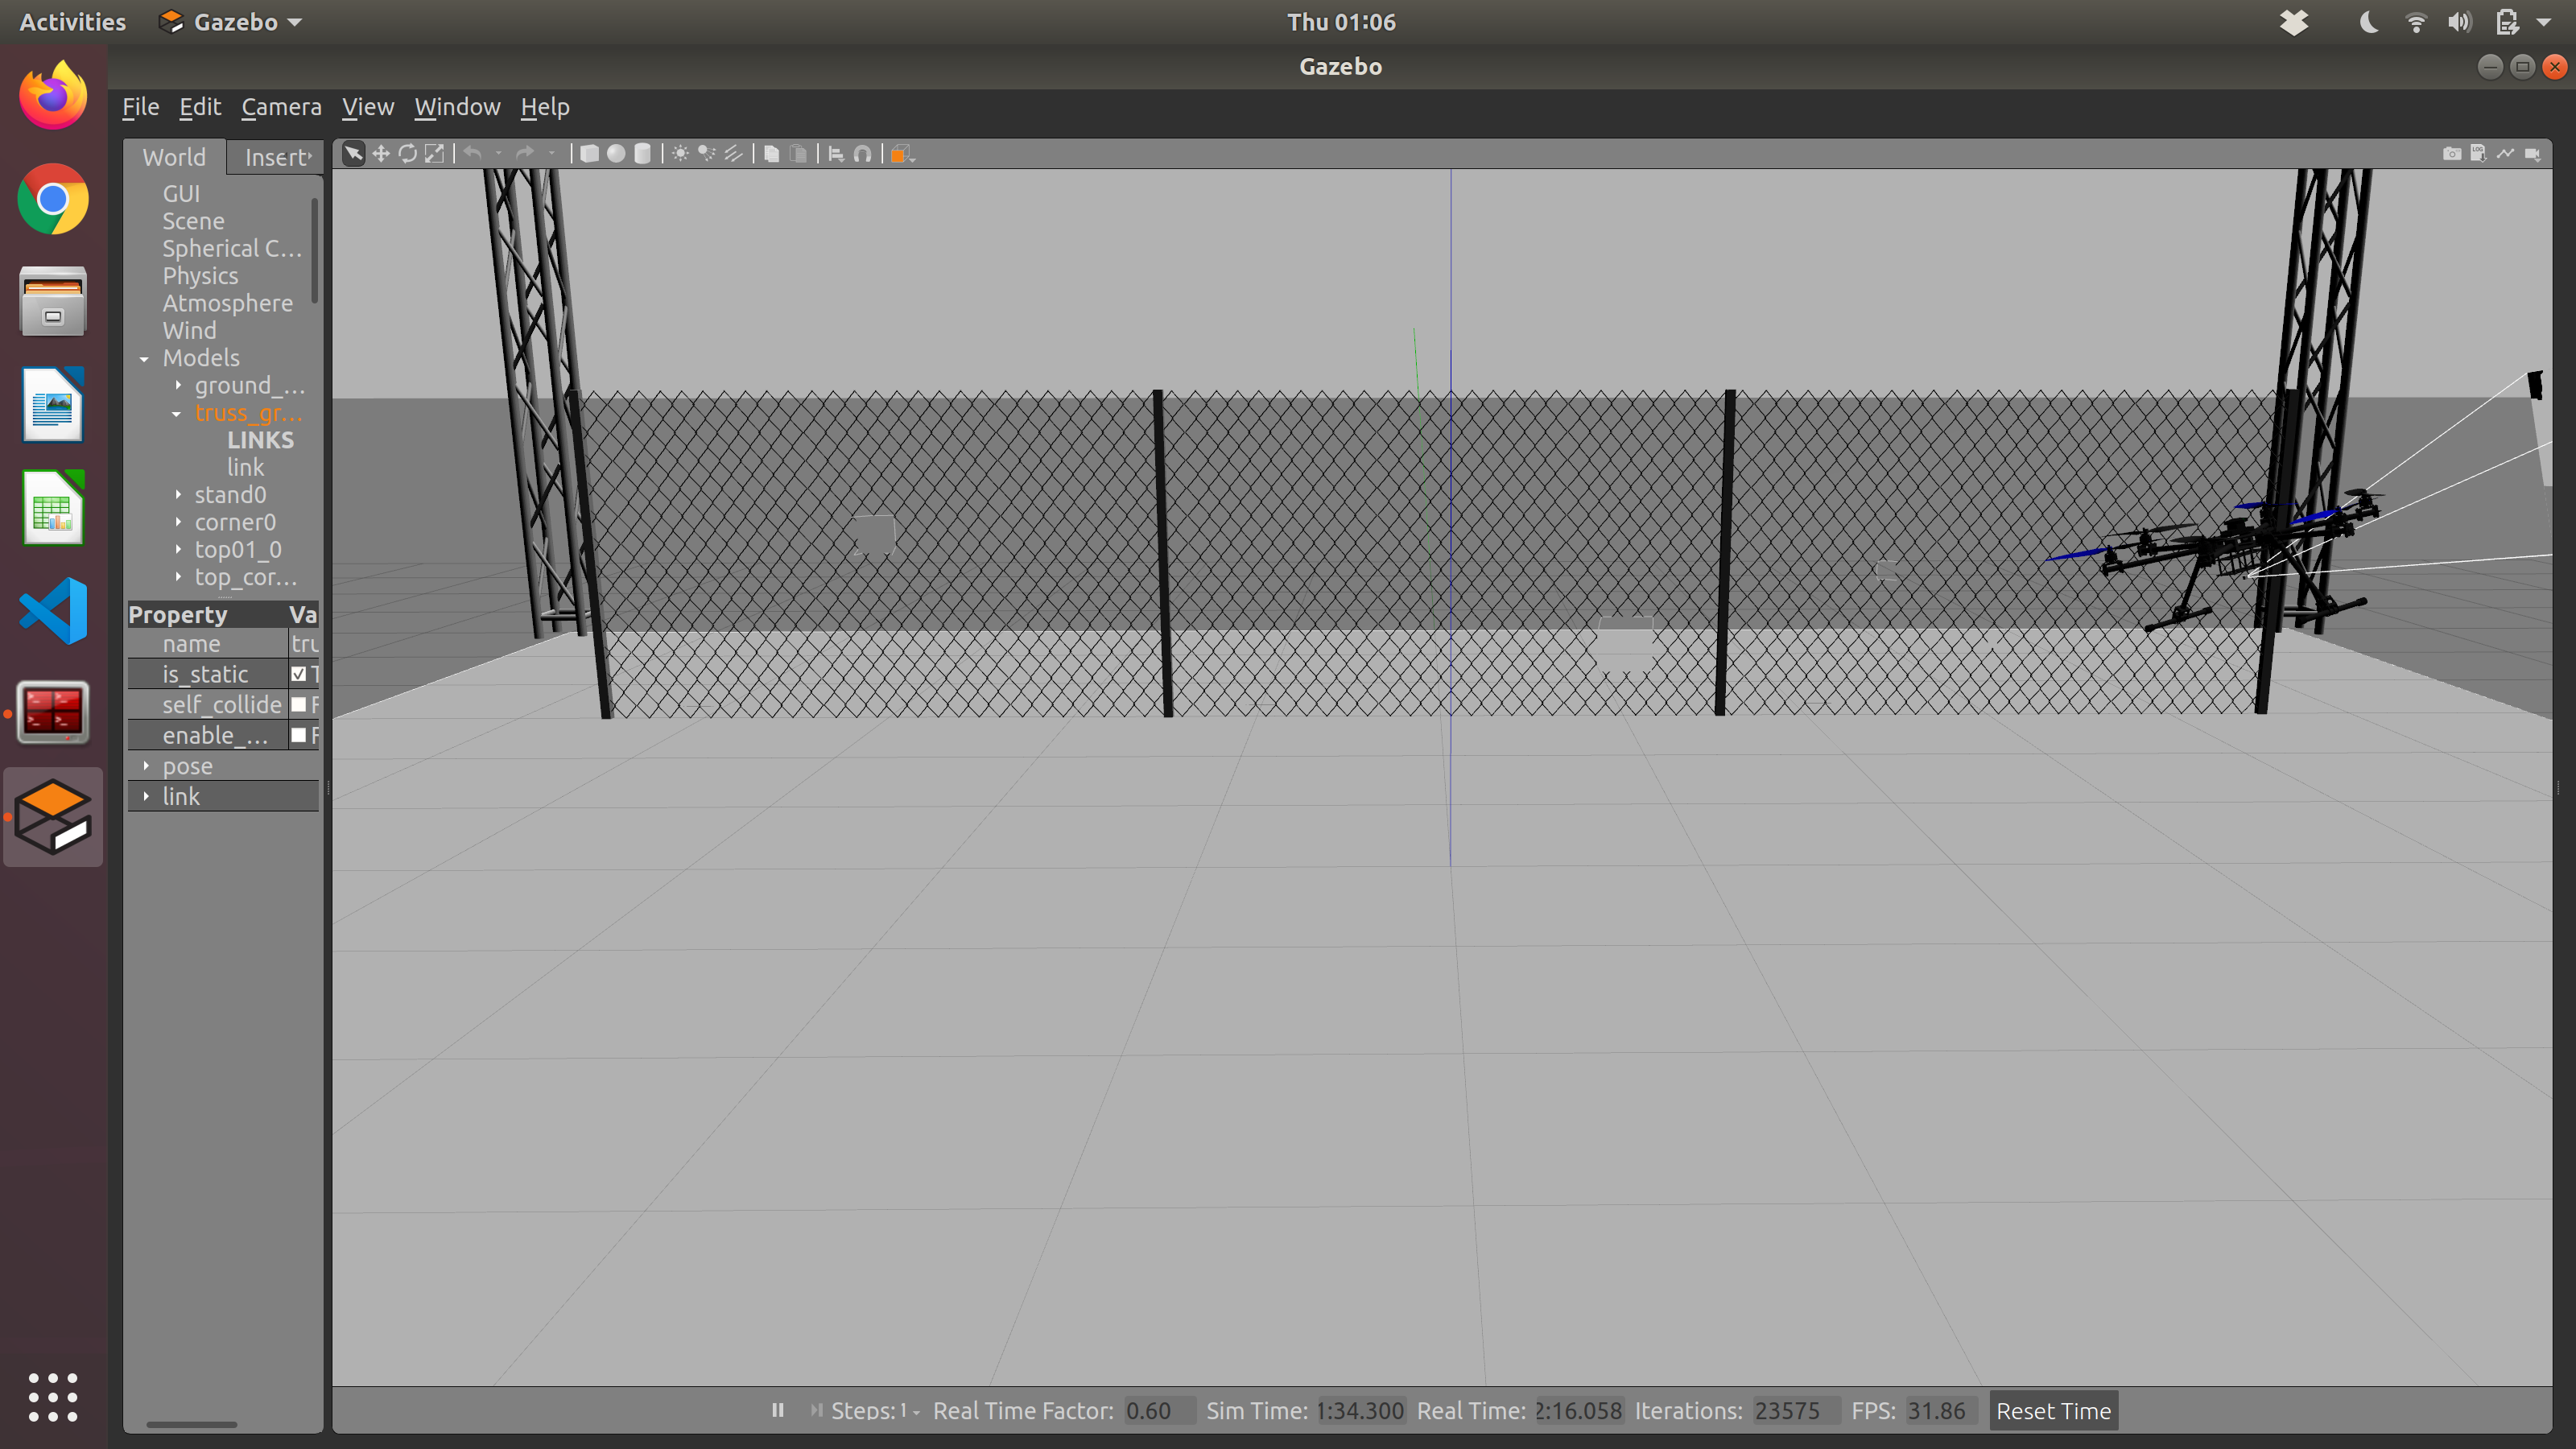
\includegraphics[width=\textwidth]{../Figures/simulation/Simulation_08.png}
        \end{subfigure}
        \begin{subfigure}{\figSize}
            \centering
            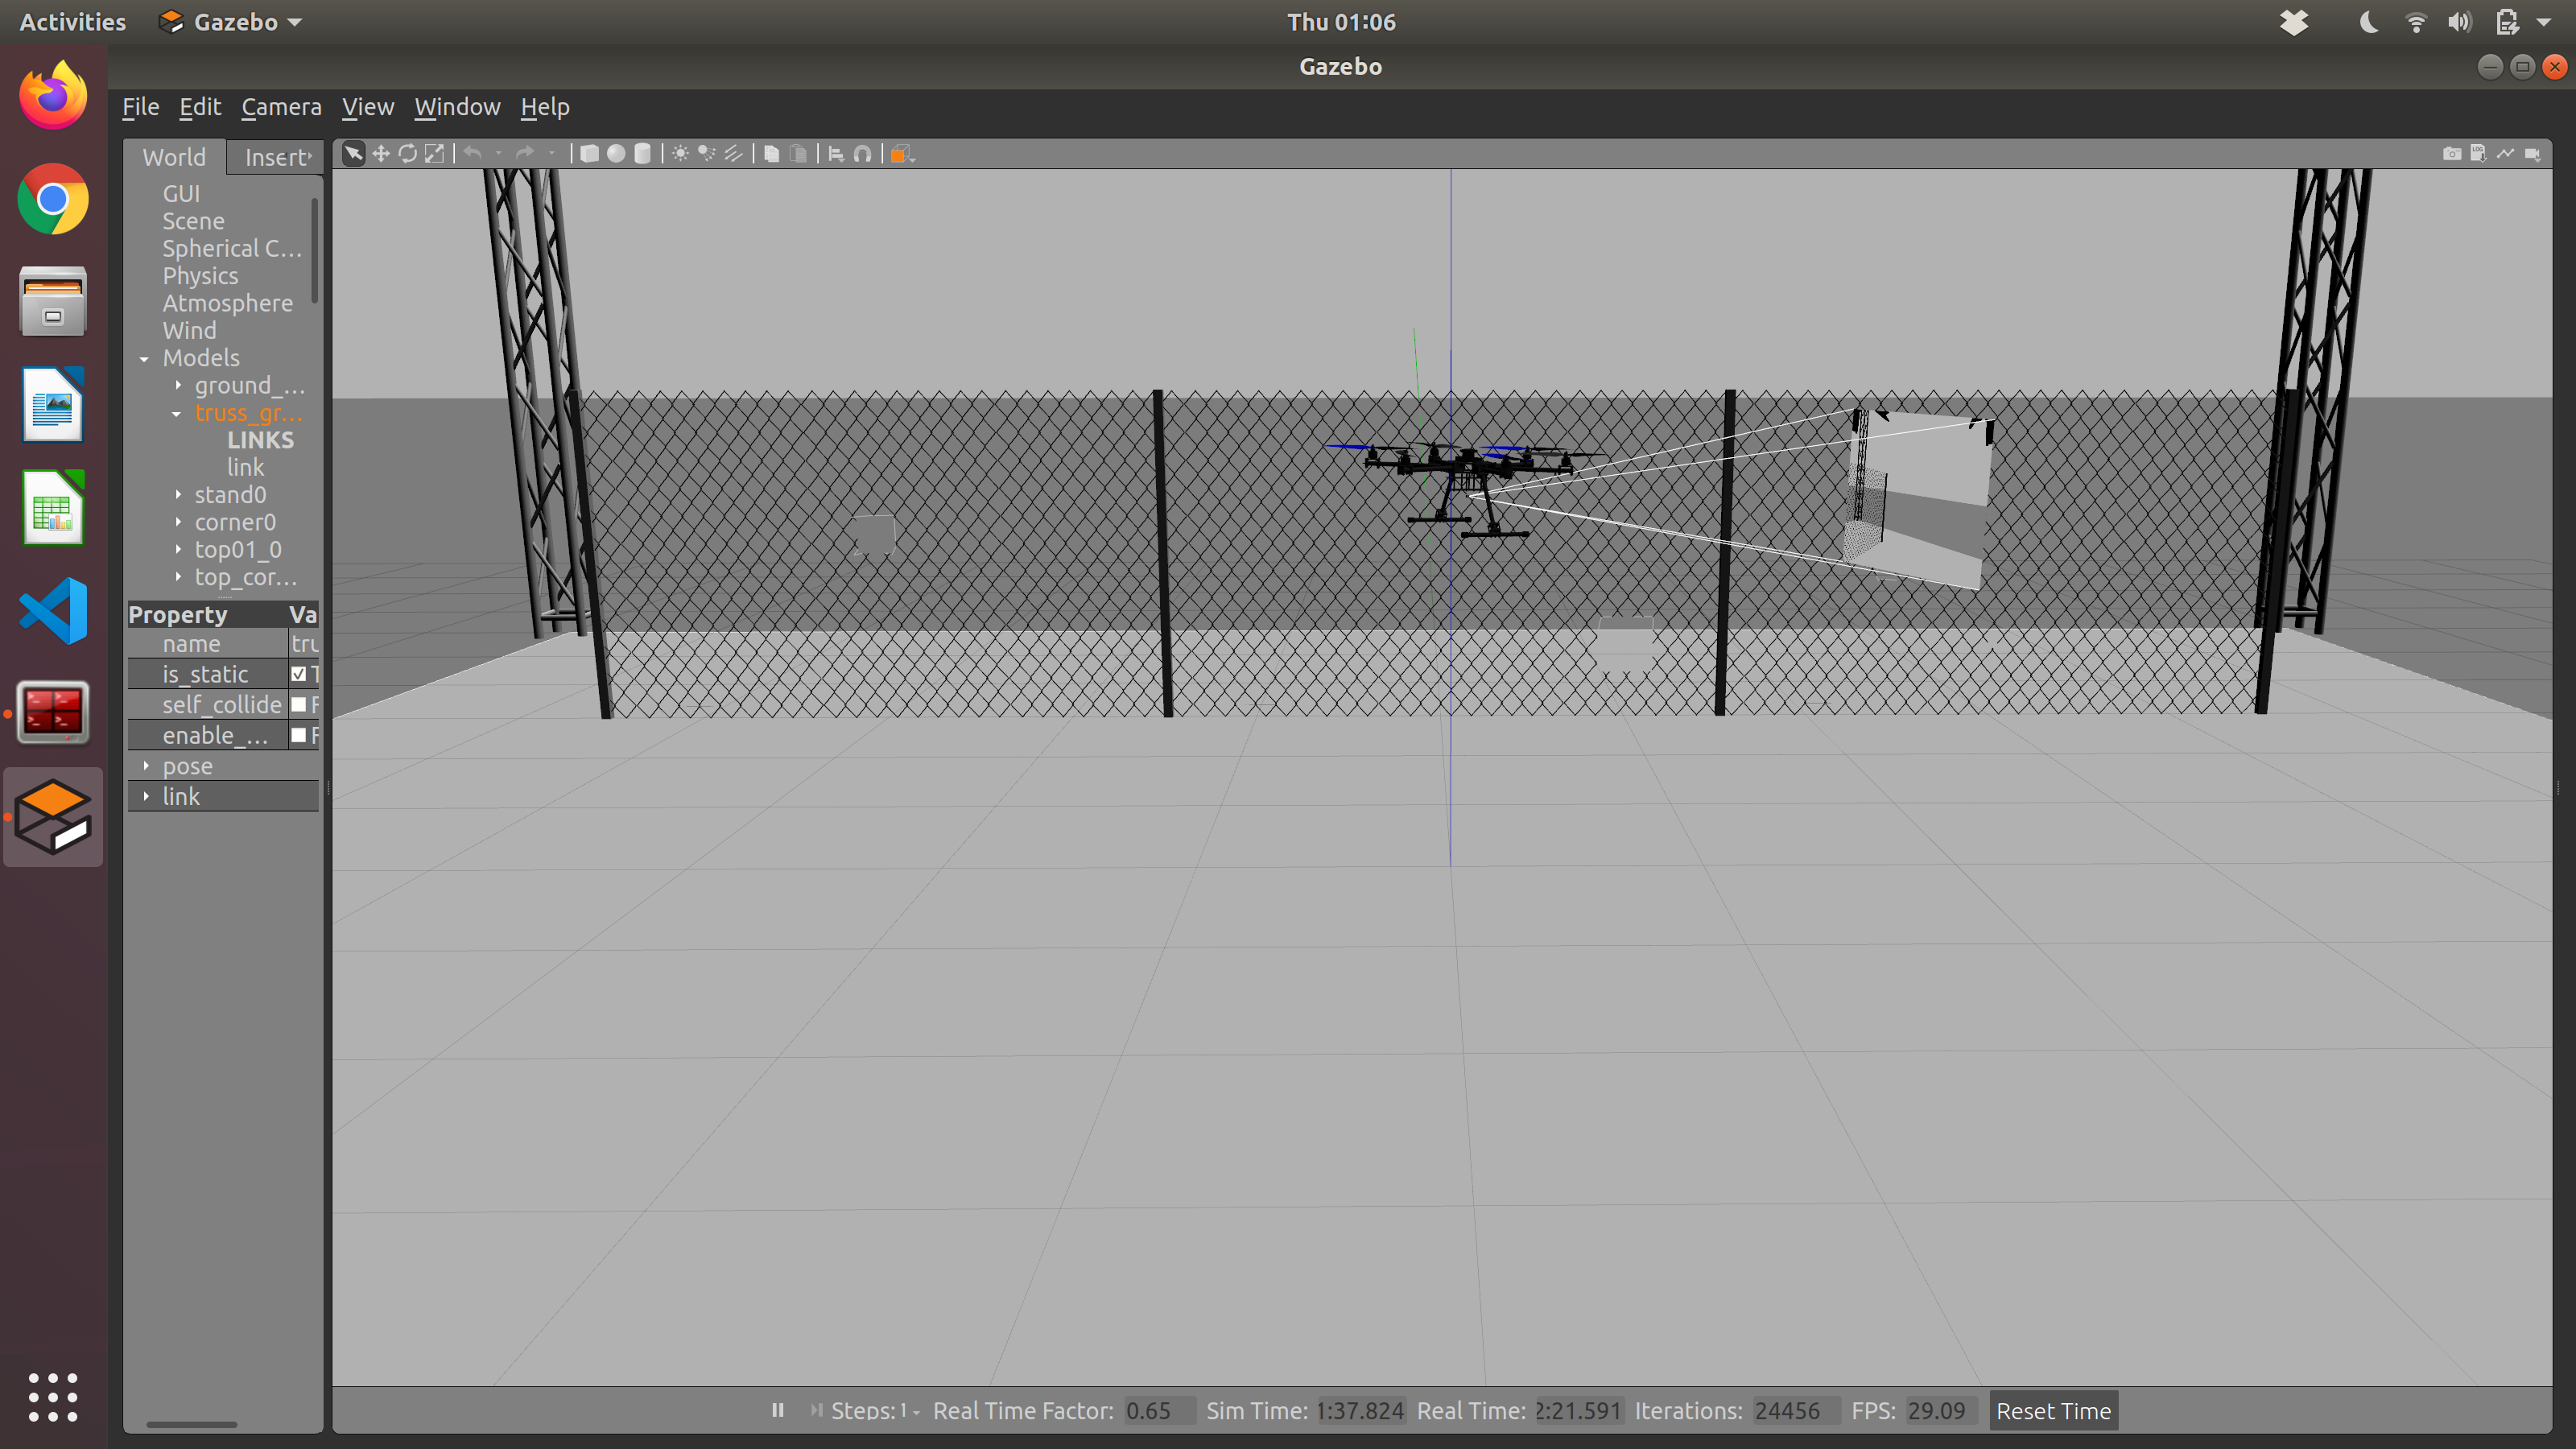
\includegraphics[width=\textwidth]{../Figures/simulation/Simulation_09.png}
        \end{subfigure}
        \begin{subfigure}{\figSize}
            \centering
            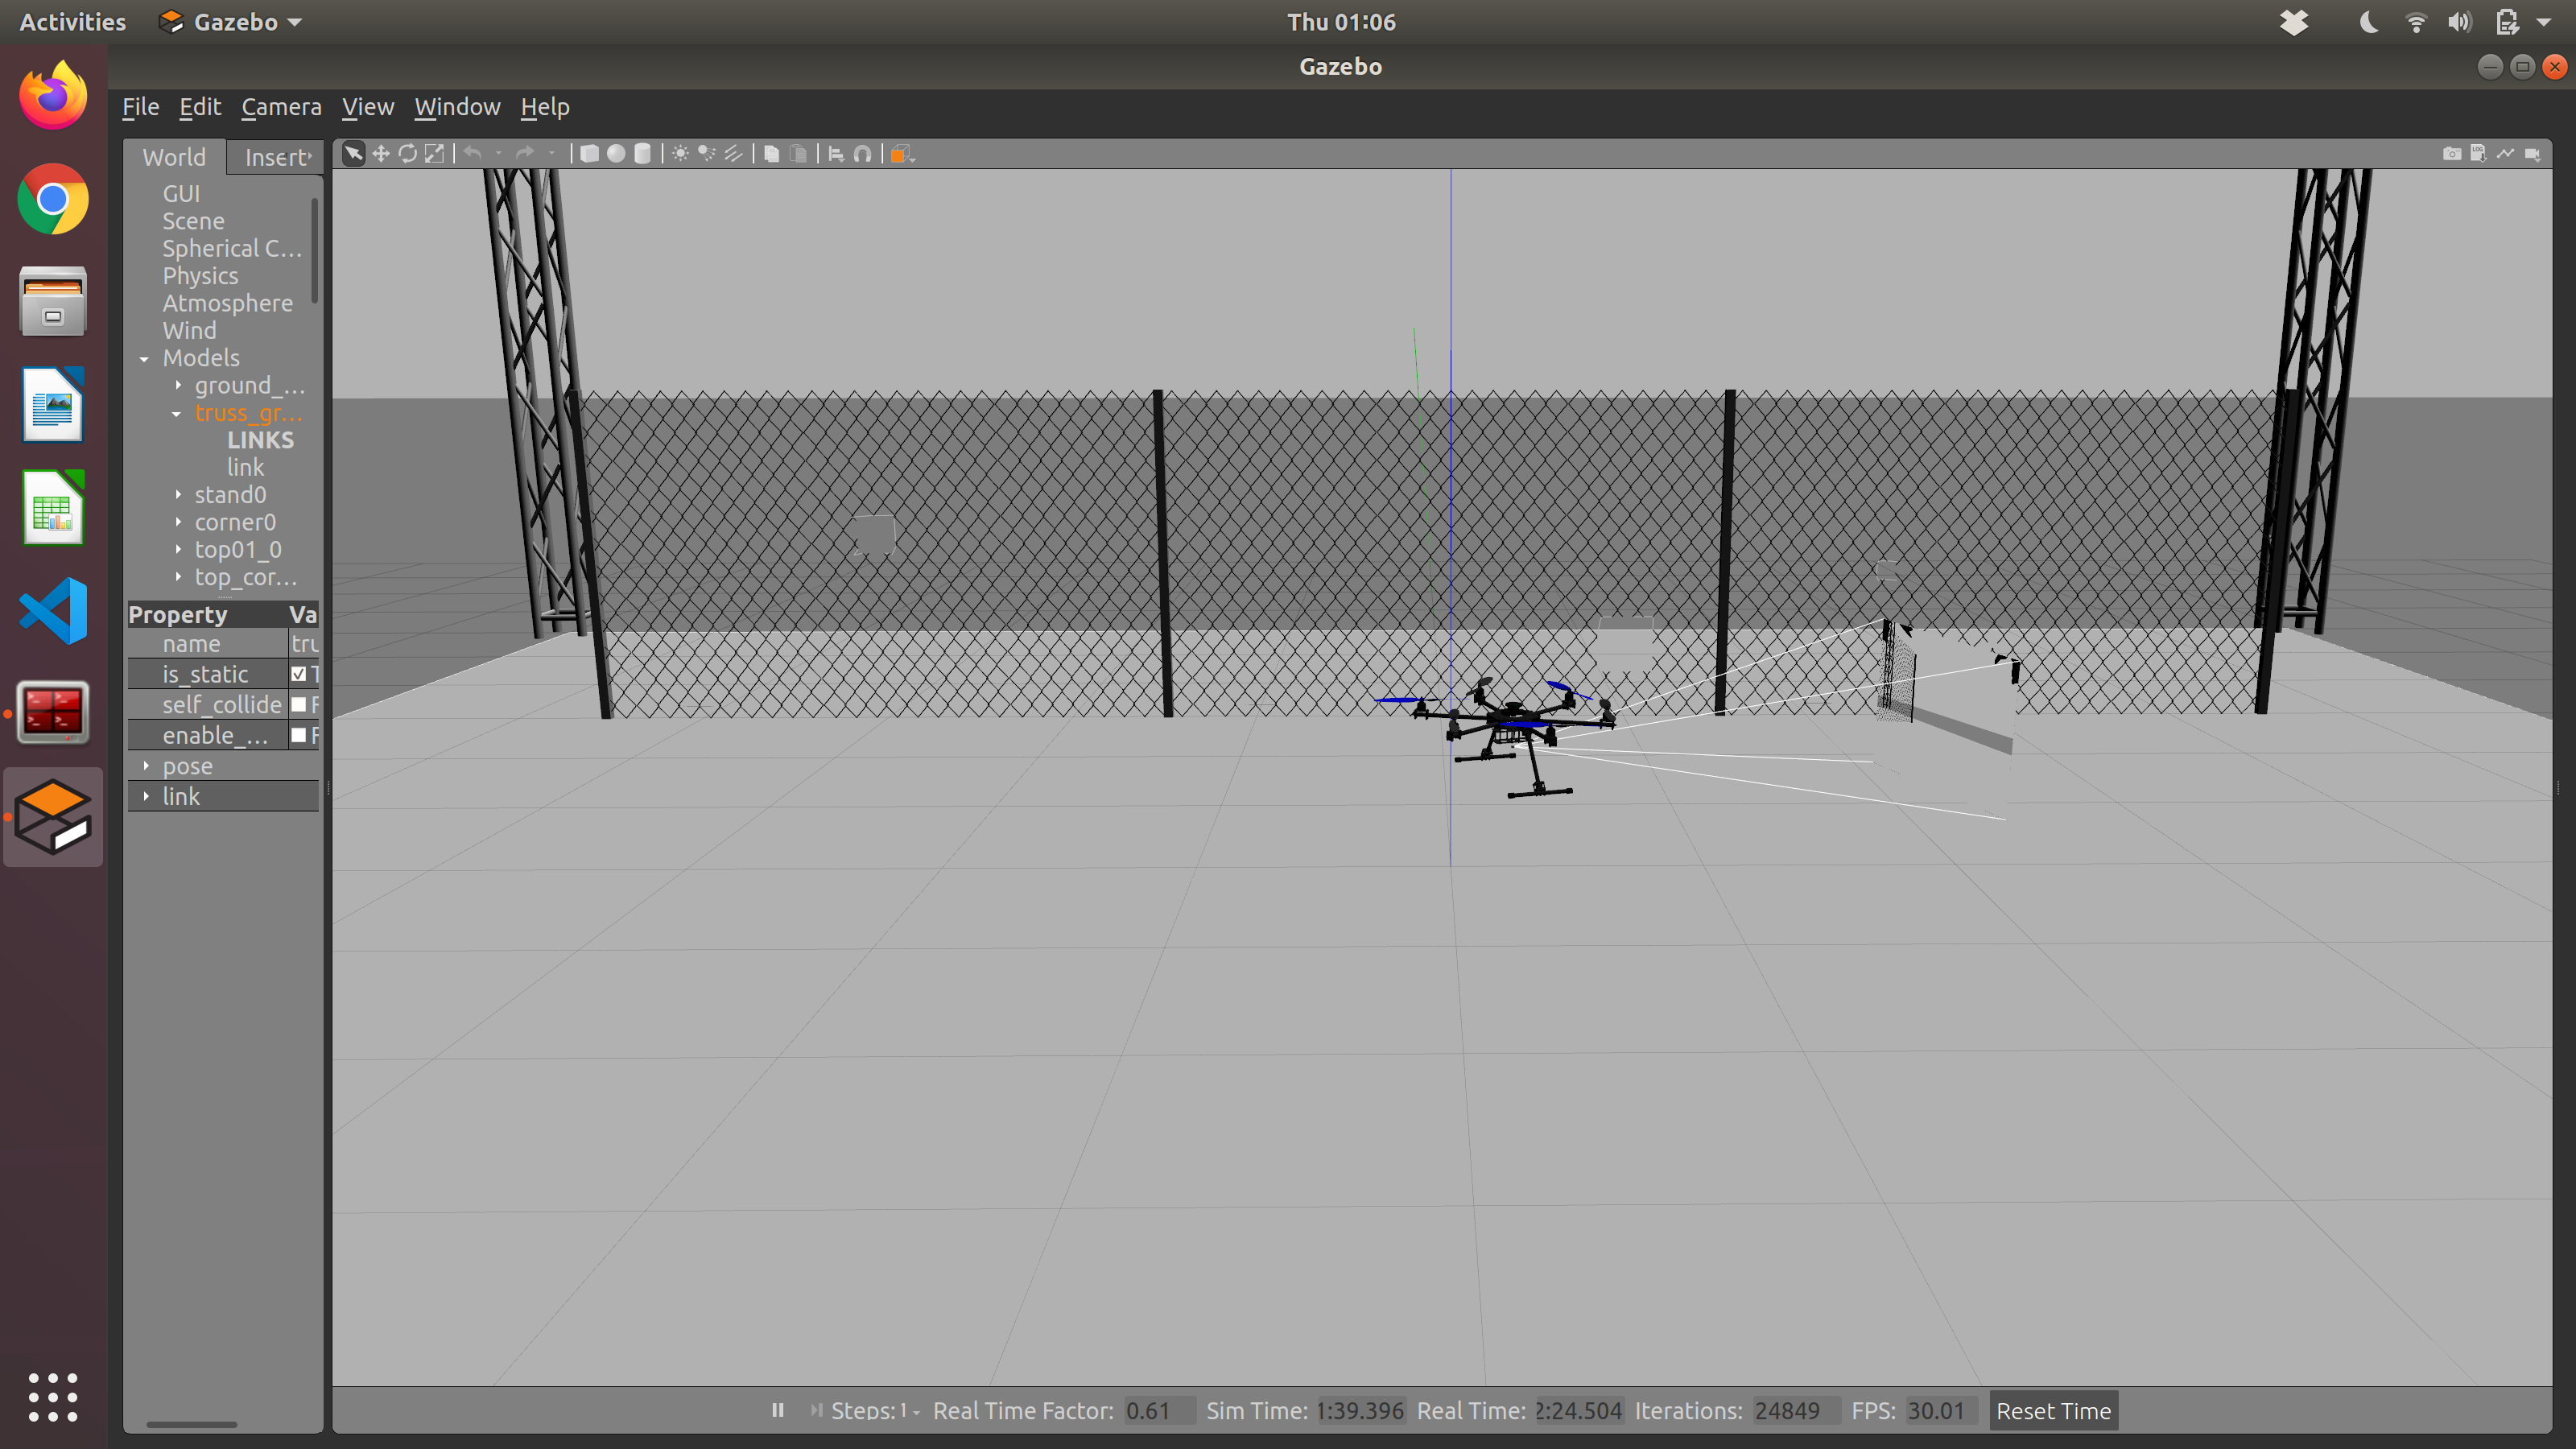
\includegraphics[width=\textwidth]{../Figures/simulation/Simulation_10.png}
        \end{subfigure}
        \begin{subfigure}{\figSize}
            \centering
            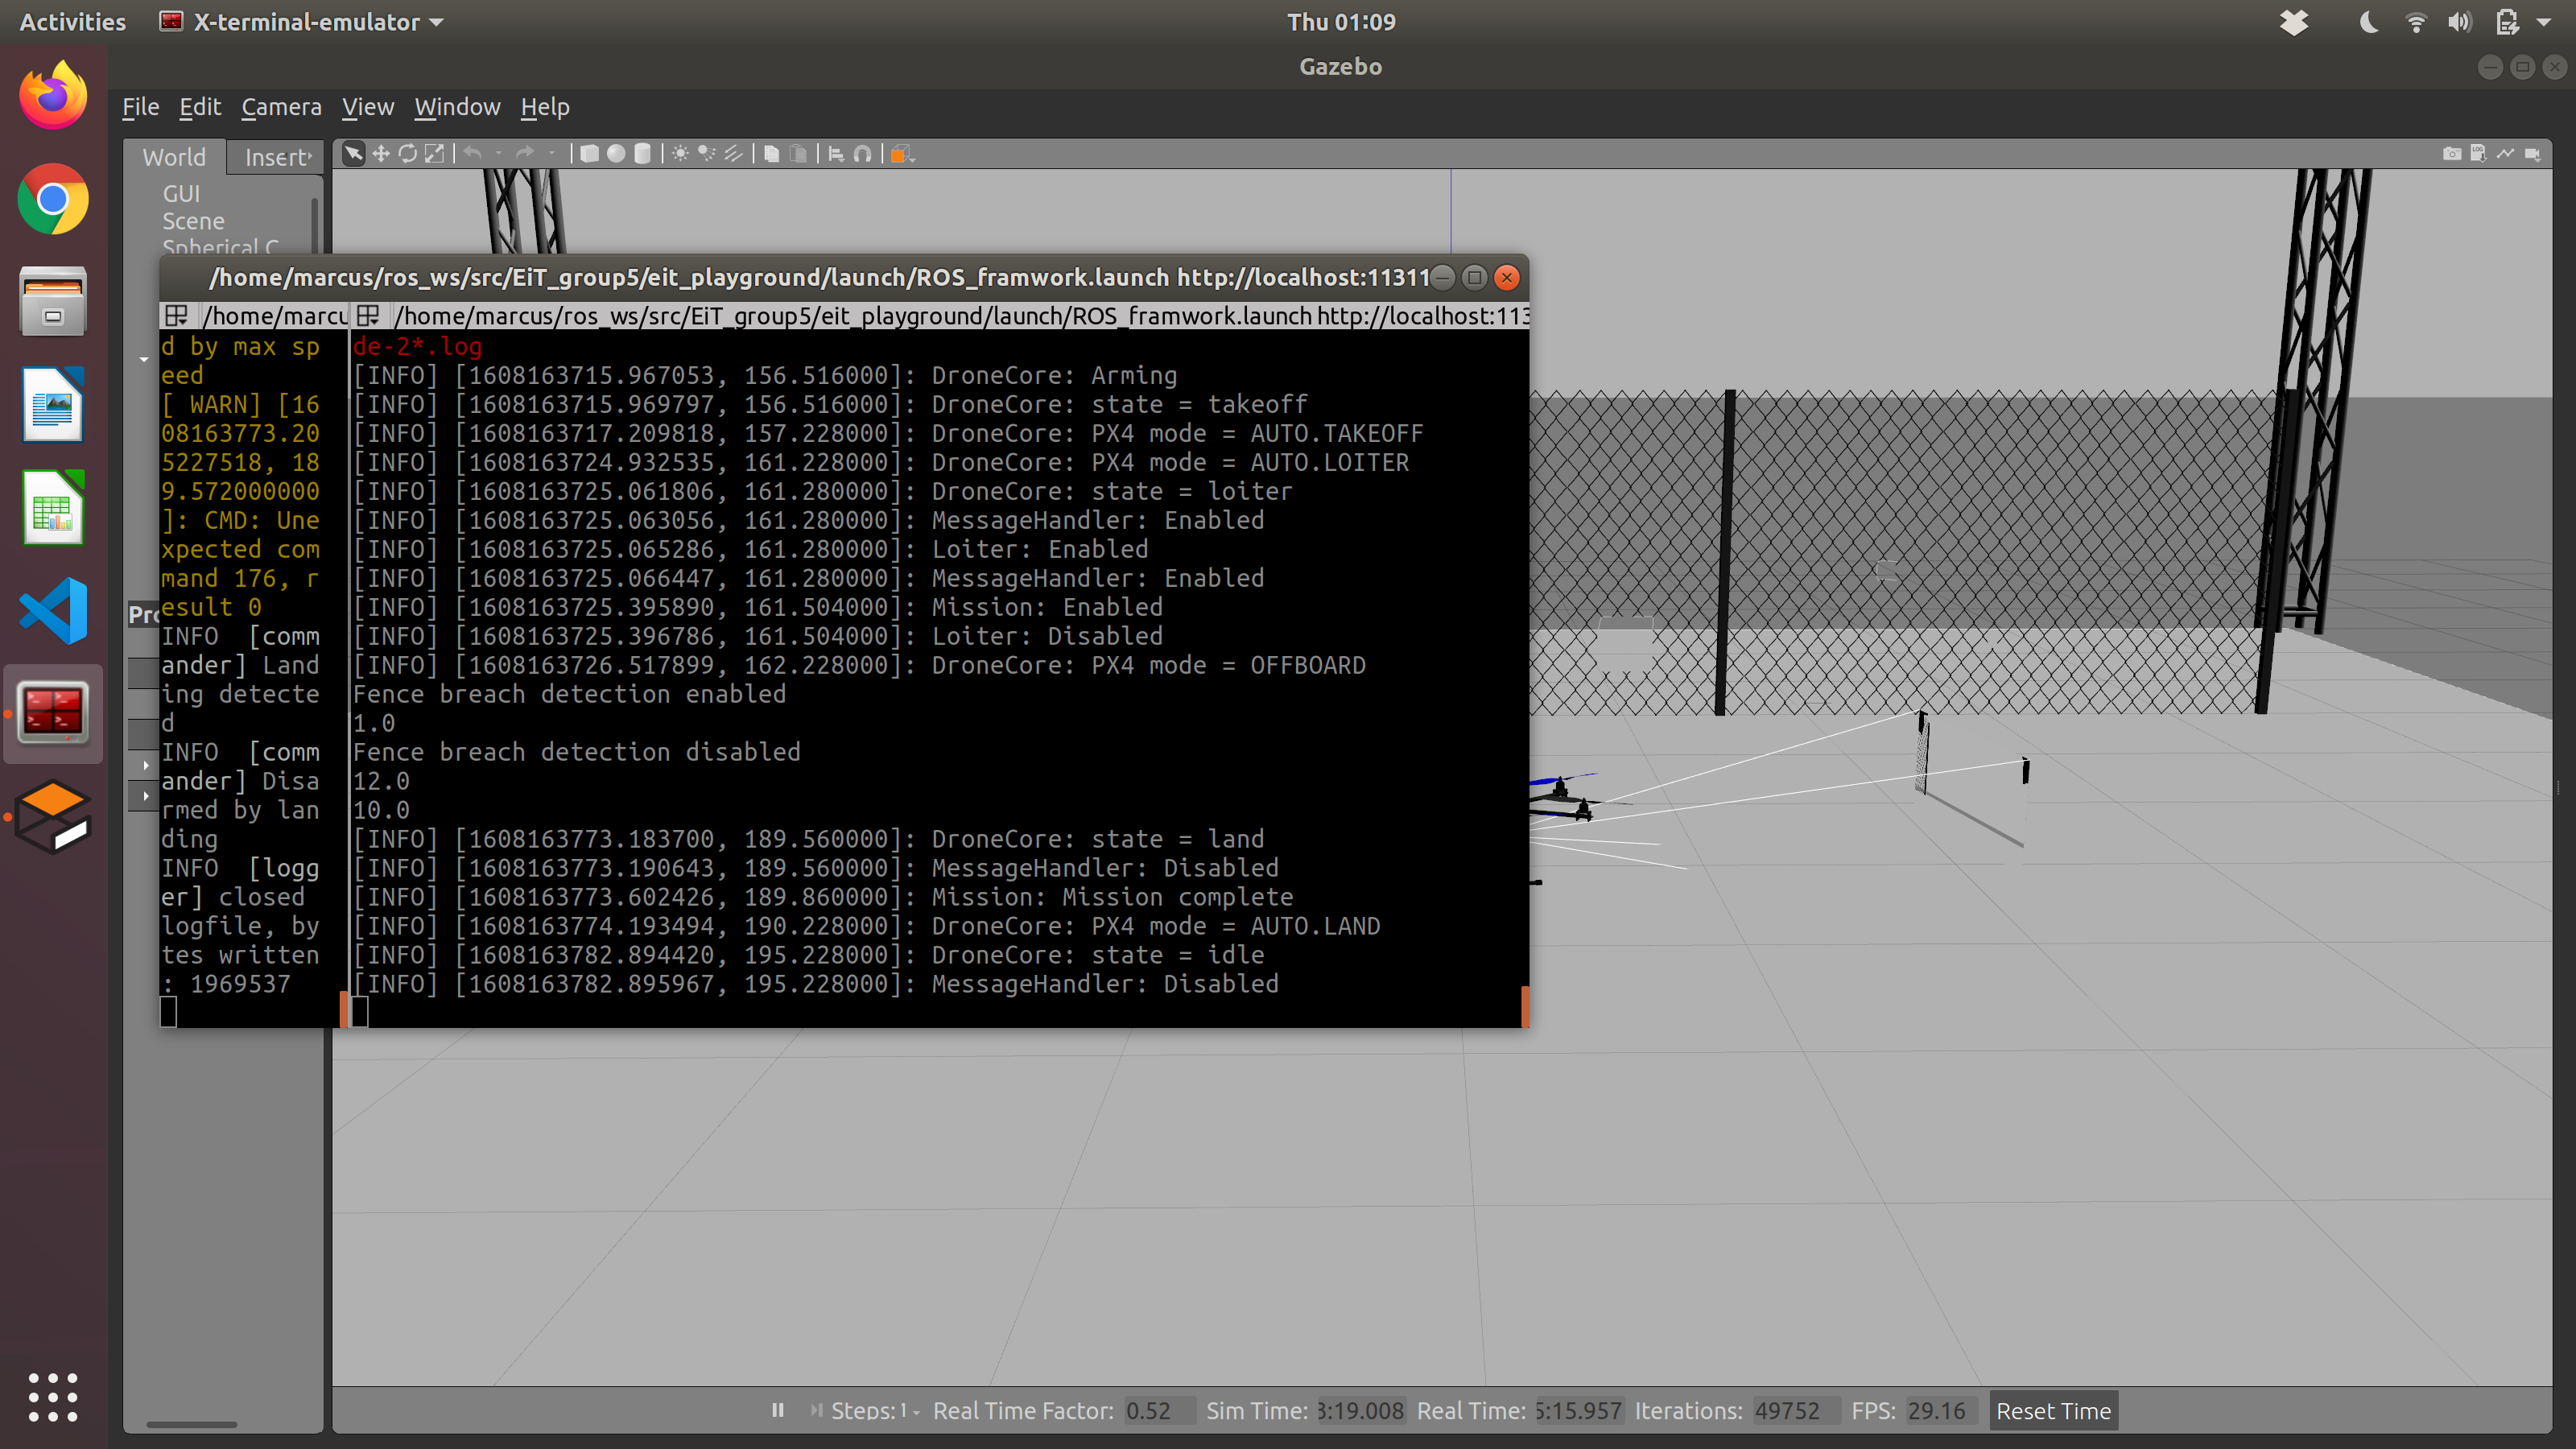
\includegraphics[width=\textwidth]{../Figures/simulation/Simulation_11.png}
        \end{subfigure}  
        \caption{Illustration of a simple autonomous flight in the Gazebo simulation}
        \label{fig:SIM_flight}
\end{figure}



\end{document}